\chapter{Testowanie i eksperymenty}

Testowanie, porównywanie sposobu działania poszczególnych plannerów a także tworzenie różnych próbnych scenariuszy stanowiło najważniejszy cel realizowanego projektu. To wszystko miało służyć wykreowaniu swoistego oglądu sytuacji jakie sposoby kontroli są najoptymalniejsze, jakie nadają się do konkretnych zastosowań, a także co składa się na ich słabe strony. Przeprowadzone testy miały służyć również zobrazowaniu możliwości MoveIta. W tym celu zaproponowano szereg eksperymentów, których wyniki zestawiono w poniższych podrozdziałach. By móc zbierać konkretne pomiary napisano w tym celu kilka skryptów w języku Python. Byli to klasyczni subskrybenci ROS, którzy zapisywali pożądane wartości do plików csv. W dalszej kolejności na ich podstawie generowano wykresy, tabele itp.

\section{Porównanie planerów}

\subsection{Czas planowania}
Jednym z pierwszych testów jakie przeprowadzono było porównanie czasów planowania trasy przez poszczególne plannery. W tym celu przygotowano dwa osobne scenariusze. W pierwszym z nich trasa do pokonania była bardzo prosta. Robot musiał poruszyć jedynie jednym złączem. Planowanie trasy dla każdego algorytmu powtarzano 10 krotnie, tak by na końcu móc policzyć średni czas procesu. Wielokrotne pomiary miały na celu pominięcie kwestii możliwego chwilowego obciążenia komputera wskutek wykonywania np. obsługiwanego przerwania. Kolejną rzeczą jest, iż czas planowania będzie różny przy wykorzystaniu innego komputera do obliczeń, niemniej różnice między plannerami pozostaną.

Poniższa tabela \ref{tab:10} prezentuje zebrane dane. Każdy algorytm miał do wyznaczenia trasę od pozycji pobazowej (wszystkie złącza 0$^\circ$) do pozycji w której ramię drugie opuszczone było o 35$^\circ$. Pozostałe złącza bez zmian.
 Należy podkreślić, iż eksperymenty te były prowadzone na domyślnych ustawieniach plannerów wygenerowanych przez program Setup Assistant. Dozwolona ilość podejść algorytmu do wyznaczenia trasy wynosiła 10. Pomiary wykonano na laptopie Lenovo Z51 z procesorem Intel i7 5500U, 8GB RAM DDR3, dyskiem SSD 1 TB Samsung QVO 870. Zainstalowany system jak wcześniej informowano to Ubuntu 20.04. W czasie testów nie były uruchomione inne zasobożerne procesy - jedynie notatnik do zapisywania pomiarów.   
% Please add the following required packages to your document preamble:
% \usepackage{multirow}
% \usepackage[table,xcdraw]{xcolor}
% If you use beamer only pass "xcolor=table" option, i.e. \documentclass[xcolor=table]{beamer}
\begin{table}[H]
\centering
\caption{Zestawienie czasów planowania ruchu ramienia drugiego przez poszczególne algorytmy}
\label{tab:10}
\begin{tabular}{|c|c|c|c|c|c|ll}
\cline{1-6}
\cellcolor[HTML]{C0C0C0}L.p. & \multicolumn{1}{l|}{\cellcolor[HTML]{C0C0C0}{\color[HTML]{000000} \begin{tabular}[c]{@{}l@{}}Grupa \\ plannerów\end{tabular}}} & \cellcolor[HTML]{C0C0C0}Planner     & \cellcolor[HTML]{C0C0C0}\begin{tabular}[c]{@{}c@{}}Min. czas\\ planowania {[}s{]}\end{tabular} & \cellcolor[HTML]{C0C0C0}\begin{tabular}[c]{@{}c@{}}Max. czas\\ planowania {[}s{]}\end{tabular} & \cellcolor[HTML]{C0C0C0}\begin{tabular}[c]{@{}c@{}}Średni czas \\ 10 prób {[}s{]}\end{tabular} &  &  \\ \cline{1-6}
\cellcolor[HTML]{EFEFEF}1.   & CHOMP                                                                                                                          & \cellcolor[HTML]{EFEFEF}CHOMP       & \cellcolor[HTML]{EFEFEF}0.253                                                                  & \cellcolor[HTML]{EFEFEF}0.313                                                                  & \cellcolor[HTML]{EFEFEF}0.267                                                                  &  &  \\ \cline{1-6}
\cellcolor[HTML]{C0C0C0}2.   &                                                                                                                                & \cellcolor[HTML]{C0C0C0}BFMT        & \cellcolor[HTML]{C0C0C0}1.164                                                                  & \cellcolor[HTML]{C0C0C0}0.959                                                                  & \cellcolor[HTML]{C0C0C0}1.027                                                                  &  &  \\ \cline{1-1} \cline{3-6}
\cellcolor[HTML]{FFCCC9}3.   &                                                                                                                                & \cellcolor[HTML]{FFCCC9}BKPIECE     & \cellcolor[HTML]{FFCCC9}2.565                                                                  & \cellcolor[HTML]{FFCCC9}-                                                                      & \cellcolor[HTML]{FFCCC9}2.565                                                                  &  &  \\ \cline{1-1} \cline{3-6}
\cellcolor[HTML]{9AFF99}4.   &                                                                                                                                & \cellcolor[HTML]{9AFF99}BiEST       & \cellcolor[HTML]{9AFF99}0.037                                                                  & \cellcolor[HTML]{9AFF99}0.048                                                                  & \cellcolor[HTML]{9AFF99}0.042                                                                  &  &  \\ \cline{1-1} \cline{3-6}
\cellcolor[HTML]{9AFF99}5.   &                                                                                                                                & \cellcolor[HTML]{9AFF99}BiTRRT      & \cellcolor[HTML]{9AFF99}0.020                                                                  & \cellcolor[HTML]{9AFF99}0.029                                                                  & \cellcolor[HTML]{9AFF99}0.023                                                                  &  &  \\ \cline{1-1} \cline{3-6}
\cellcolor[HTML]{C0C0C0}6.   &                                                                                                                                & \cellcolor[HTML]{C0C0C0}EST         & \cellcolor[HTML]{C0C0C0}0.070                                                                  & \cellcolor[HTML]{C0C0C0}0.185                                                                  & \cellcolor[HTML]{C0C0C0}0.121                                                                  &  &  \\ \cline{1-1} \cline{3-6}
\cellcolor[HTML]{EFEFEF}7.   &                                                                                                                                & \cellcolor[HTML]{EFEFEF}FMT         & \cellcolor[HTML]{EFEFEF}0.892                                                                  & \cellcolor[HTML]{EFEFEF}0.965                                                                  & \cellcolor[HTML]{EFEFEF}0.925                                                                  &  &  \\ \cline{1-1} \cline{3-6}
\cellcolor[HTML]{C0C0C0}8.   &                                                                                                                                & \cellcolor[HTML]{C0C0C0}KPIECE      & \cellcolor[HTML]{C0C0C0}0.109                                                                  & \cellcolor[HTML]{C0C0C0}0.270                                                                  & \cellcolor[HTML]{C0C0C0}0.155                                                                  &  &  \\ \cline{1-1} \cline{3-6}
\cellcolor[HTML]{FFCCC9}9.   &                                                                                                                                & \cellcolor[HTML]{FFCCC9}LBKPIECE    & \cellcolor[HTML]{FFCCC9}X                                                                      & \cellcolor[HTML]{FFCCC9}X                                                                      & \cellcolor[HTML]{FFCCC9}X                                                                      &  &  \\ \cline{1-1} \cline{3-6}
\cellcolor[HTML]{C0C0C0}10.  &                                                                                                                                & \cellcolor[HTML]{C0C0C0}LBTRRT      & \cellcolor[HTML]{C0C0C0}0.102                                                                  & \cellcolor[HTML]{C0C0C0}-                                                                      & \cellcolor[HTML]{C0C0C0}0.102                                                                  &  &  \\ \cline{1-1} \cline{3-6}
\cellcolor[HTML]{FFCCC9}11.  &                                                                                                                                & \cellcolor[HTML]{FFCCC9}LazyPRM     & \cellcolor[HTML]{FFCCC9}X                                                                      & \cellcolor[HTML]{FFCCC9}X                                                                      & \cellcolor[HTML]{FFCCC9}X                                                                      &  &  \\ \cline{1-1} \cline{3-6}
\cellcolor[HTML]{C0C0C0}12.  &                                                                                                                                & \cellcolor[HTML]{C0C0C0}LazyPRMstar & \cellcolor[HTML]{C0C0C0}0.101                                                                  & \cellcolor[HTML]{C0C0C0}-                                                                      & \cellcolor[HTML]{C0C0C0}0.101                                                                  &  &  \\ \cline{1-1} \cline{3-6}
\cellcolor[HTML]{EFEFEF}13.  &                                                                                                                                & \cellcolor[HTML]{EFEFEF}PDST        & \cellcolor[HTML]{EFEFEF}0.071                                                                  & \cellcolor[HTML]{EFEFEF}0.228                                                                  & \cellcolor[HTML]{EFEFEF}0.138                                                                  &  &  \\ \cline{1-1} \cline{3-6}
\cellcolor[HTML]{C0C0C0}14.  &                                                                                                                                & \cellcolor[HTML]{C0C0C0}PRM         & \cellcolor[HTML]{C0C0C0}0.057                                                                  & \cellcolor[HTML]{C0C0C0}0.119                                                                  & \cellcolor[HTML]{C0C0C0}0.085                                                                  &  &  \\ \cline{1-1} \cline{3-6}
\cellcolor[HTML]{EFEFEF}15.  &                                                                                                                                & \cellcolor[HTML]{EFEFEF}PRMstar     & \cellcolor[HTML]{EFEFEF}0.101                                                                  & \cellcolor[HTML]{EFEFEF}-                                                                      & \cellcolor[HTML]{EFEFEF}0.101                                                                  &  &  \\ \cline{1-1} \cline{3-6}
\cellcolor[HTML]{C0C0C0}16.  &                                                                                                                                & \cellcolor[HTML]{C0C0C0}ProjEST     & \cellcolor[HTML]{C0C0C0}0.064                                                                  & \cellcolor[HTML]{C0C0C0}0.197                                                                  & \cellcolor[HTML]{C0C0C0}0.139                                                                  &  &  \\ \cline{1-1} \cline{3-6}
\cellcolor[HTML]{9AFF99}11.  &                                                                                                                                & \cellcolor[HTML]{9AFF99}RRTConnect  & \cellcolor[HTML]{9AFF99}0.22                                                                   & \cellcolor[HTML]{9AFF99}0.046                                                                  & \cellcolor[HTML]{9AFF99}0.036                                                                  &  &  \\ \cline{1-1} \cline{3-6}
\cellcolor[HTML]{C0C0C0}12.  &                                                                                                                                & \cellcolor[HTML]{C0C0C0}RRT         & \cellcolor[HTML]{C0C0C0}0.032                                                                  & \cellcolor[HTML]{C0C0C0}0.080                                                                  & \cellcolor[HTML]{C0C0C0}0.516                                                                  &  &  \\ \cline{1-1} \cline{3-6}
\cellcolor[HTML]{EFEFEF}13.  &                                                                                                                                & \cellcolor[HTML]{EFEFEF}RRTstar     & \cellcolor[HTML]{EFEFEF}0.101                                                                  & \cellcolor[HTML]{EFEFEF}-                                                                      & \cellcolor[HTML]{EFEFEF}0.101                                                                  &  &  \\ \cline{1-1} \cline{3-6}
\cellcolor[HTML]{FFCCC9}14.  &                                                                                                                                & \cellcolor[HTML]{FFCCC9}SBL         & \cellcolor[HTML]{FFCCC9}2.011                                                                  & \cellcolor[HTML]{FFCCC9}-                                                                      & \cellcolor[HTML]{FFCCC9}2.011                                                                  &  &  \\ \cline{1-1} \cline{3-6}
\cellcolor[HTML]{EFEFEF}15.  &                                                                                                                                & \cellcolor[HTML]{EFEFEF}SPARS       & \cellcolor[HTML]{EFEFEF}0.183                                                                  & \cellcolor[HTML]{EFEFEF}-                                                                      & \cellcolor[HTML]{EFEFEF}0.183                                                                  &  &  \\ \cline{1-1} \cline{3-6}
\cellcolor[HTML]{C0C0C0}16.  &                                                                                                                                & \cellcolor[HTML]{C0C0C0}SPARStwo    & \cellcolor[HTML]{C0C0C0}0.101                                                                  & \cellcolor[HTML]{C0C0C0}-                                                                      & \cellcolor[HTML]{C0C0C0}0.101                                                                  &  &  \\ \cline{1-1} \cline{3-6}
\cellcolor[HTML]{EFEFEF}17.  &                                                                                                                                & \cellcolor[HTML]{EFEFEF}STRIDE      & \cellcolor[HTML]{EFEFEF}0.081                                                                  & \cellcolor[HTML]{EFEFEF}0.175                                                                  & \cellcolor[HTML]{EFEFEF}0.118                                                                  &  &  \\ \cline{1-1} \cline{3-6}
\cellcolor[HTML]{9AFF99}18.  & \multirow{-23}{*}{OMPL}                                                                                                        & \cellcolor[HTML]{9AFF99}TRRT        & \cellcolor[HTML]{9AFF99}0.022                                                                  & \cellcolor[HTML]{9AFF99}0.047                                                                  & \cellcolor[HTML]{9AFF99}0.033                                                                  &  &  \\ \cline{1-6}
\cellcolor[HTML]{9AFF99}19.  &                                                                                                                                & \cellcolor[HTML]{9AFF99}PTP         & \cellcolor[HTML]{9AFF99}0.000                                                                  & \cellcolor[HTML]{9AFF99}0.001                                                                  & \cellcolor[HTML]{9AFF99}0.001                                                                  &  &  \\ \cline{1-1} \cline{3-6}
\cellcolor[HTML]{9AFF99}20.  & \multirow{-2}{*}{\begin{tabular}[c]{@{}c@{}}Pilz Industrial \\ Motion Planner\end{tabular}}                                    & \cellcolor[HTML]{9AFF99}LIN         & \cellcolor[HTML]{9AFF99}0.004                                                                  & \cellcolor[HTML]{9AFF99}0.007                                                                  & \cellcolor[HTML]{9AFF99}0.005                                                                  &  &  \\ \cline{1-6}
\end{tabular}
\end{table}
Wnioski jakie nasuwają się po przeanalizowaniu powyższego zestawienia to fakt, iż różnice w czasach planowania istotnie występują. Wiele plannerów osiąga zbliżone czasy, natomiast część znacząco odbiega od pozostałych. 

Dla prostego zadania, jakim było poruszenie jednym złączem grupa plannerów wchodzących w skład Pilz Industrial Motion Planner wydaje się być bezkonkurencyjna. Ścieżkę otrzymywano praktycznie natychmiast. Ze względu na opisywaną w rozdziale drugim prostotę tych algorytmów świetnie nadają się one do takowych zastosowań. 

Najlepsze z algorytmów wchodzących w skład grupy OMPL również okazały się całkiem szybkie. Planowanie trasy zajmowało średnio od dwóch do czterech setnych sekundy. 

Dziwi natomiast fakt, iż plannery takie jak LBKPIECE oraz LazyPRM nie były w stanie w ogóle zaplanować trasy. Pierwszy z wymienionych spowodował zawieszenie się programu Rviz (prawdopodobnie wystąpił błąd). Natomiast w drugim przypadku pomimo zwiększenia maksymalnego czasu planowania do 60 sekund - wyniku nie otrzymano.

W przeprowadzonych eksperymentach bardzo źle wypadł również planner BKPIECE. Najniższy odnotowany czas planowania (ponad 2.5 sekundy) udało się zaobserwować tylko raz. Pozostałe czasy przekraczały zazwyczaj dwukrotnie tę wartość. Dodatkowo bardzo często przy wybraniu zbyt niskiej maksymalnej długości czasu planowania, zabieg ten w ogóle się nie udawał. Planowanie trajektorii kończyło się błędem (nie znajdowano trasy w dopuszczalnym czasie). 

Zauważono, że algorytmy posiadające w nazwie człon $star$ (chociaż nie tylko) charakteryzowało specyficzne zachowanie. Wykorzystywały one cały określony przez użytkownika maksymalny czas planowania, próbując znaleźć najlepsze możliwe rozwiązanie. Dopiero po upływie tego czasu wybierały optymalną znalezioną trajektorię. Często minimalny potrzebny do zaplanowania czas wynosił jedną dziesiątą sekundy (czyli minimum możliwe do ustalenia w Rviz), niemniej zdarzało się, iż potrzebowały one tego czasu więcej (np. algorytm SBL, który potrzebował minimum 2 sekund na znalezienie trasy). W takich przypadkach nie należy opierać swoich założeń, o wyznaczony minimalny czas, gdyż nie jest on powtarzalny. Oznacza to, iż przykładowo na dziesięć prób, raz uda się uzyskać taki czas, natomiast w pozostałych przypadkach proces zakończy się niepowodzeniem. Dlatego w praktyce minimalny czas dający gwarancję otrzymania wyniku będzie dwu lub nawet trzykrotnie większy.

Zauważono również, iż w przypadku plannera CHOMP, mimo umiarkowanych czasów planowania jakie otrzymywano, cały proces od momentu jego uruchomienia do zwrócenia wyniku był znacząco dłuższy od wskazywanego. Odnosi się zatem wrażenie jakoby spore znaczenie miało również wywołanie i obsługa plannera, a nie tylko sam proces działania algorytmu wyznaczającego trasę. W przypadku plannerów OMPL i Pilz nie zaobserwowano takiej tendencji.

%Dzieje się tak, ze względu na sposób ustalania minimalnego czasu planowania dla takich algorytmów. Stosowano system 10 prób. Jeżeli dla zadanego czasu maksymalnego planowania (np. 2 sekund) dziesięć razy z rzędu wyznaczanie trasy kończyło się niepowodzeniem, wówczas uznawano, iż algorytm nie jest w stanie zaplanować ruchu w tak krótkim czasie. 



W dalszej kolejności postanowiono powtórzyć test jednak z uwzględnieniem konieczności przemieszczenia wszystkich złącz. Chciano w ten sposób sprawdzić czy dla plannera ma znaczenie ile osi musi ustawić. Jednak w tym eksperymencie postanowiono pominąć już algorytmy, które w poprzednim zestawieniu wypadły najsłabiej. 

Wyniki zaprezentowano poniżej (wykres \ref{fig:30}), zestawiając ze sobą średni czas 10 prób przy planowaniu ruchu jednej oraz wszystkich osi. W ten sposób możliwe jest zaobserwowanie ewentualnej różnicy. Pomiary dla jednej osi zaczerpnięto z poprzedniego eksperymentu (\ref{tab:4}). Natomiast w przypadku pomiarów wszystkich osi, ich nastawy były kolejno: 90$^\circ$ wieża, -10$^\circ$ ram. główne, -20$^\circ$ ram. drugie, 90$^\circ$ ram. trzecie, 30$^\circ$ obrót chwytaka. W każdym przypadku dozwolona ilość podejść algorytmu do wyznaczenia trasy wynosiła 10. 

 \begin{figure}[H]
	\centering
	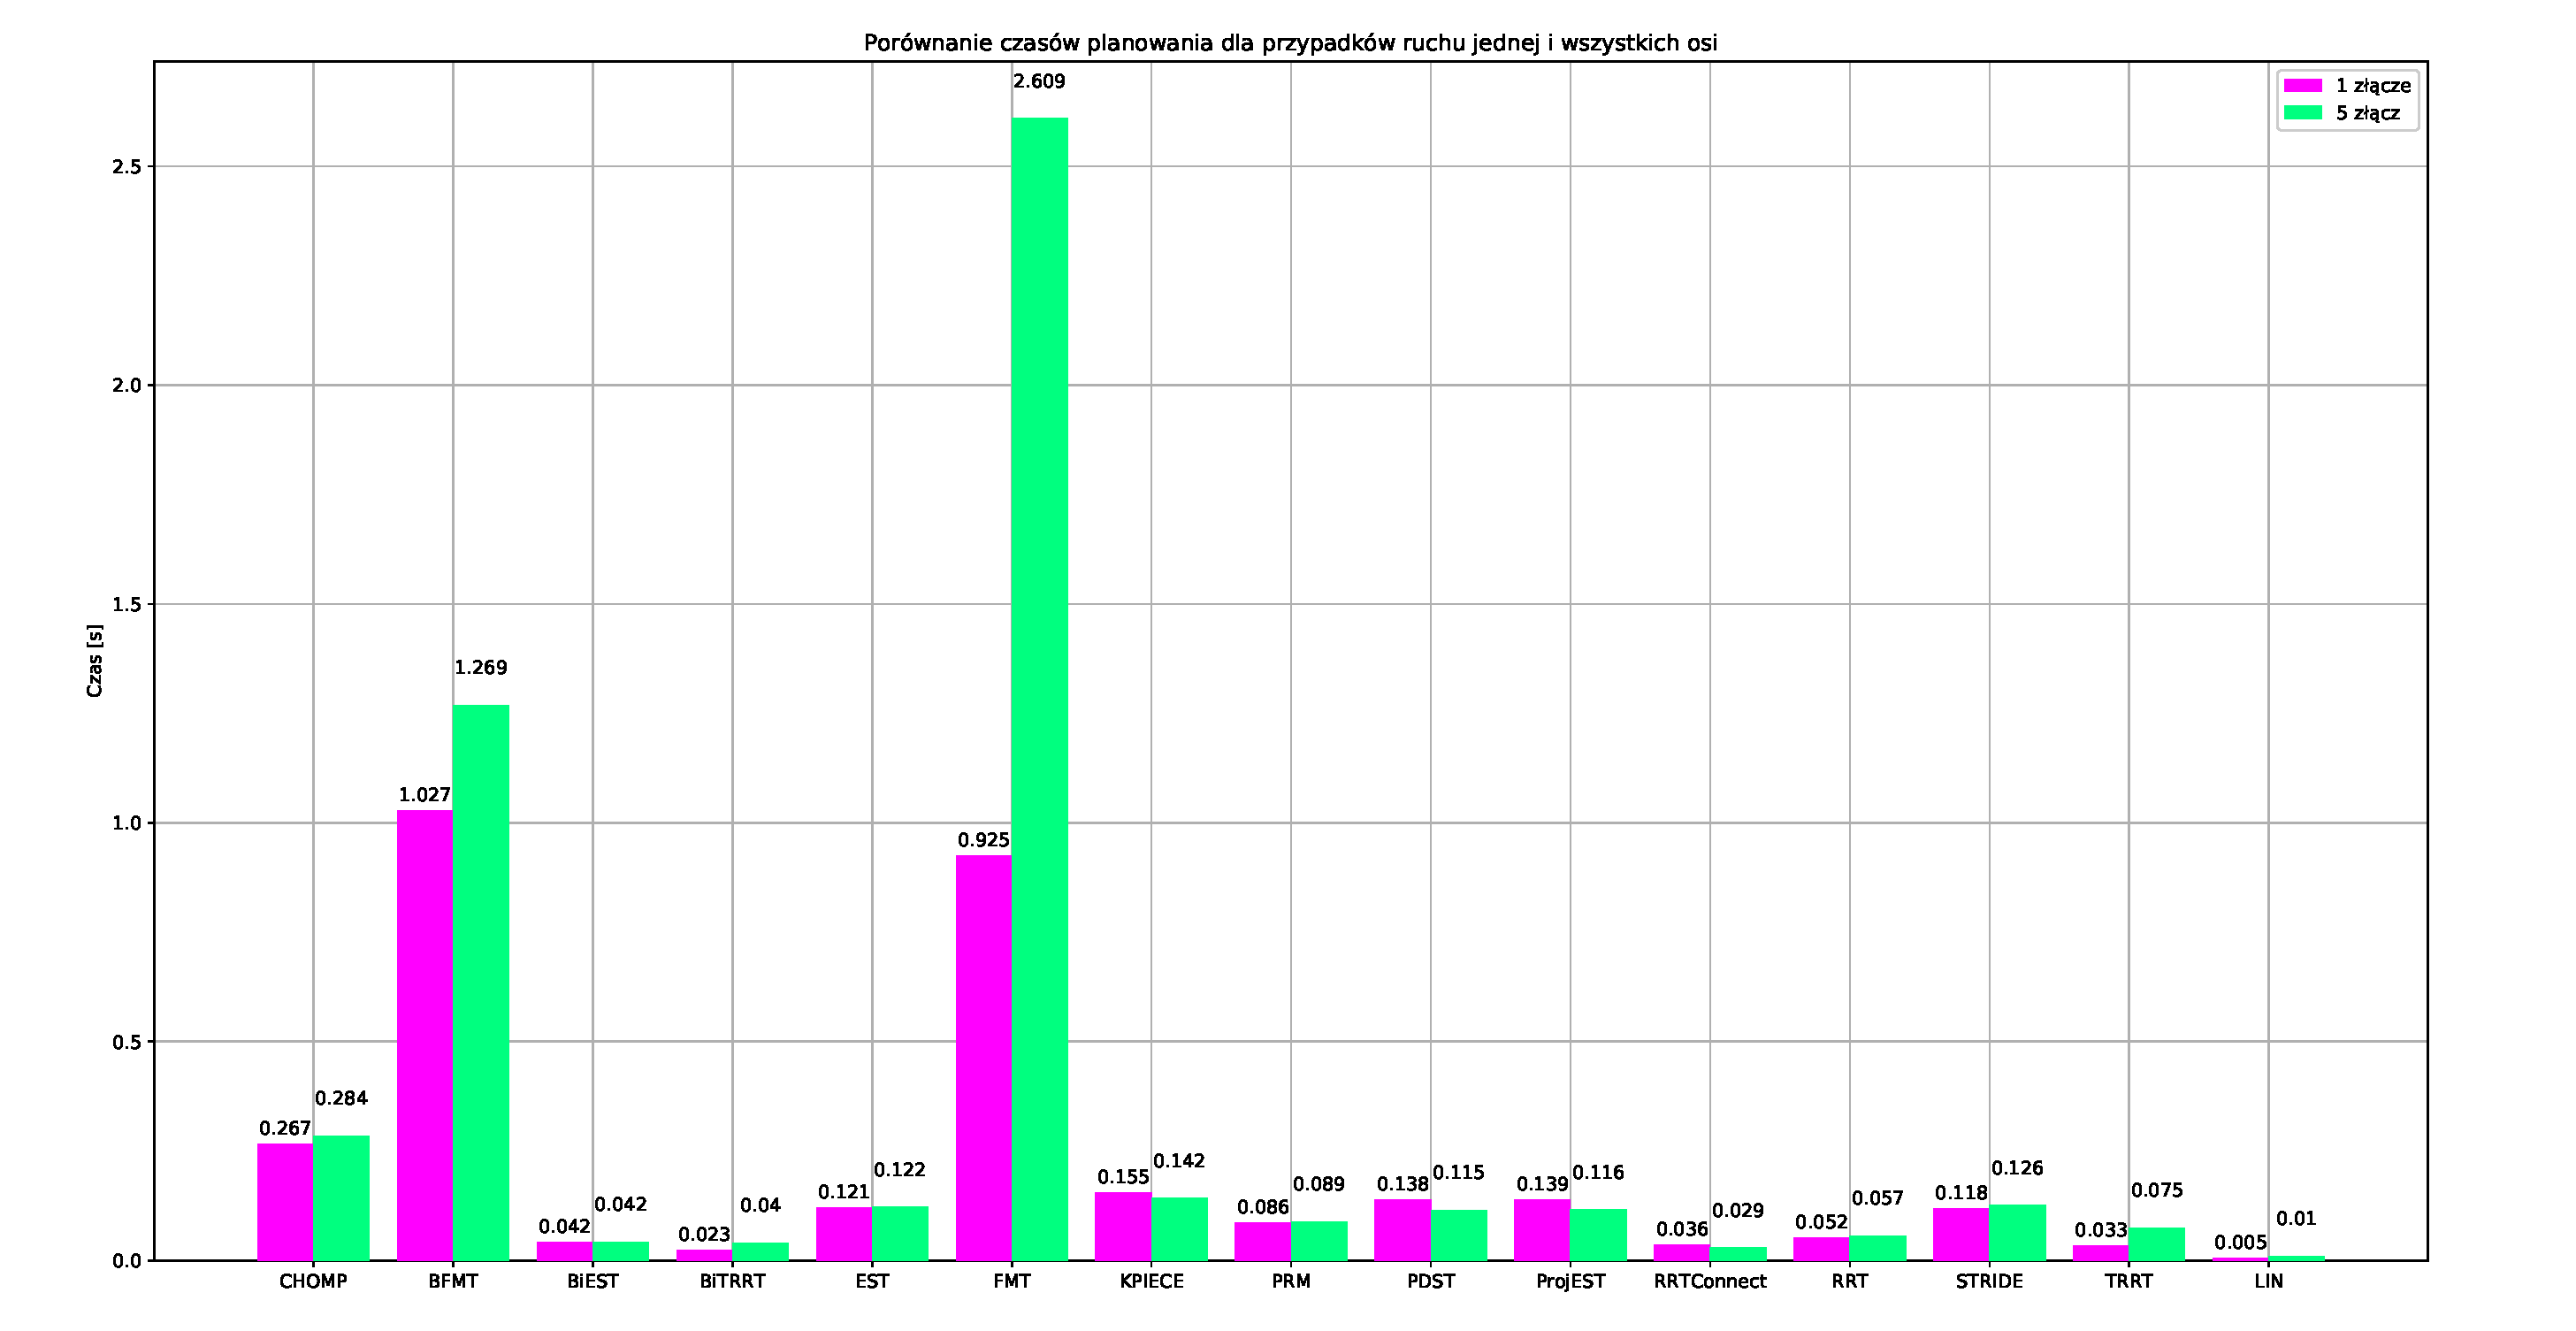
\includegraphics[width=0.9\linewidth]{{img/Figure_com.eps}}
	\caption{Porównanie czasów planowania dla przypadku ruchu jednej i wszystkich osi.}
	\label{fig:30}
\end{figure}

Powyższy wykres uwidacznia fakt, iż zasadniczo dla dwóch plannerów - BFMT oraz FMT ma znaczenie ile członów robota muszą przemieścić. Szczególnie w przypadku algorytmu FMT różnica jest ogromna. Względnie dużą zmianę odnotowano także w przypadku algorytmów BiEST, BiTRRT, TRRT oraz LIN. Mimo nawet dwukrotnemu wydłużeniu procesu planowania, czasy przez nie uzyskiwane nadal pozostają na bardzo dobrym poziomie. Natomiast jeżeli chodzi o pozostałe plannery, to różnice są raczej niewielkie. Czasami wręcz na korzyść wszystkich złącz, niemniej na tyle subtelne, iż raczej nie stwierdzano by na ich podstawie jednoznacznej tendencji. Warto również zaznaczyć, iż w porównaniu nie uwzględniono algorytmu Pilz PTP, gdyż w jego sytuacji nie odnotowano żadnej różnicy w czasie wyznaczania trasy.

Jak wcześniej informowano - wszystkie dotychczas przeprowadzane eksperymenty dotyczyły sytuacji dla 10 dozwolonych prób planowania trasy przez algorytm. Postanowiono zatem sprawdzić jak dopuszczalna ilość tych prób przekłada się na czas wygenerowania trasy. 

Wyniki zestawiono na poniższym wykresie słupkowym. Jak wcześniej pominięto niektóre z najsłabszych algorytmów oraz te wykorzystujące cały dopuszczalny czas planowania. Sprawdzano czasy planowania dla ograniczenia 1 podejścia, 10 oraz 20. Jak i poprzednio każda z zaprezentowanych na zestawieniu wartości stanowi średnią z 10 różnych pomiarów. Przemieszczenie złącz było identyczne jak w poprzednim teście - wymagany ruch wszystkich osi robota.

 \begin{figure}[H]
	\centering
	\includegraphics[width=0.9\linewidth]{{img/Figure_att_2.eps}}
	\caption{Porównanie czasów planowania dla różnej dozwolonej maksymalnej ilości prób.}
	\label{fig:31}
\end{figure}

Analizując powyższy wykres można wyróżnić na nim pewne grupy plannerów. W pierwszej z grup powinny się znaleźć takie algorytmy jak CHOMP, PRM oraz PDST. Są to plannery, dla których czasy planowania nie zależą od ilości dopuszczalnych podejść do wyznaczenia trasy. Za każdym razem otrzymywane wyniki były bardzo zbliżone. Nie dało się stwierdzić jednoznacznej tendencji. Kolejną grupę stanowi pozostała większość algorytmów, które mogąc podejść kilkukrotnie do wyznaczenia trasy, czynią to. Wydaje się, iż najgorzej w zestawieniu tym wypadają BFMT oraz KPIECE gdzie czas drastycznie się wydłuża. Przy czym jest to pewnie spowodowane faktem, iż po prostu wykorzystują dostępną możliwość wielu prób i poszukują najbardziej optymalnego rozwiązania. Takie zachowanie może być pożądane w trudniejszych zastosowaniach, wymagających np. ominięcia przeszkody. W rozpatrywanym przypadku nie daje zbyt wielu korzyści.


Wyżej wspominano, iż wszystkie prowadzone do tej pory eksperymenty zostały przeprowadzone dla domyślnie wygenerowanych nastaw plannerów. Jednak chcąc przedstawić całościowy obraz sytuacji, postanowiono sprawdzić jak modyfikacja niektórych  współczynników wpływa na otrzymywane rezultaty.
Wśród wielu parametrów możliwych do modyfikowania dla poszczególnych plannerów, jednym z podstawowych jest współczynnik odpowiadający za dokładność.

 \begin{figure}[H]
	\centering
	\includegraphics[width=0.9\linewidth]{{img/Figure_bias.eps}}
	\caption{Porównanie czasów planowania dla różnej zadanej dokładności (goal bias)}
	\label{fig:73}
\end{figure}

Jak można było się spodziewać - większa dokładność, wydłuża czas niezbędny na znalezienie trasy. Przy czym zależność ta jest różna dla poszczególnych plannerów. Mimo wszystko najkorzystniej wypadły dwa algorytmy - RRT oraz TRRT. Można zauważyć, iż w ich przypadkach stukrotny wzrost pożądanej dokładności, przełożył się na dziesięciokrotne wydłużenie czasu planowania (stosunek 1:10). Co jest całkiem dobrym wynikiem, zważywszy na fakt, iż dla algorytmu KPIECE zależność ta była prawie jak 1:2. 


O ile w przypadku używanego w projekcie robota precyzja zaplanowanej trasy, ze względu na mechaniczne luzy złącz, jest kwestią drugorzędną, o tyle w przypadku profesjonalnych zastosowań może stanowić kluczowy czynnik. 

Podsumowując zaprezentowane w tej sekcji wyniki eksperymentów można powiedzieć, iż każdy z algorytmów charakteryzował się specyficznymi cechami. Wydaje się, iż w przypadku prostego  zadania jakim było zwyczajne przemieszczenie wszystkich złącz optymalne pod względem czasu planowania wydają się algorytmy Pilz Industrial, gdzie wynik był praktycznie natychmiastowy. Niemniej opisane w dalszej części rozdziału, pewne ich cechy mogą powodować ich dyskwalifikacje. Ciężko też jednoznacznie krytykowanie którykolwiek z zestawionych algorytmów, gdyż czas planowania jest tylko jednym z nielicznych parametrów plannera.



\newpage
\subsection{Sposób poruszania}
W kolejnym teście postanowiono zbadać w jaki sposób poszczególne plannery realizują trasę. Dlatego też na kolejnym wykresie porównano prędkości złącza w kolejnych chwilach trasy, tak by sprawdzić jak realizowane jest przemieszczenie. Przetestowano ruch ramienia drugiego, przemieszczenie od 0$^\circ$ do -30$^\circ$. Nastawy plannerów były domyślne.

 \begin{figure}[H]
	\centering
	\includegraphics[width=1\linewidth]{{img/Figure_vel.eps}}
	\caption{Porównanie prędkości złącza ramienia drugiego w zależności od użytego plannera. \cite{plot_file}}
	\label{fig:10}
\end{figure}

Na powyższym wykresie można dostrzec prędkości odpowiadające punktom zaplanowanym przez poszczególne algorytmy. Wszystkie plannery wchodzące w skład grupy OMPL zachowywały się identycznie toteż nie prezentowano ich z osobna. Można zauważyć, iż CHOMP charakteryzuje się bardzo gęstym planowaniem kolejnych punktów. Przez to może zapewniać najdokładniejsze prowadzenie. Najszybsze przemieszczenie wydają się realizaować plannery OMPL oraz PTP. Ciekawy jest również kształt wszystkich przebiegów. Zarówno PTP jak i CHOMP dzielą trasę na dwie części.  W pierwszym fragmencie złącza przyśpieszają, w kolejnym hamują. Nieco inaczej trasę realizują algorytmy grupy OMPL, gdzie przebieg prędkości przypomina kształtem trapez. Trajektoria wygenerowana przez planner LIN mimo, iż najdłuższa to wydaje się być dokładna, ze względu na ilość punktów. Posiada też charakterystyczny kształt.  

W kolejnym kroku postanowiono powtórzyć eksperyment, zwiększają jednak długość przemieszczenia. Chciano w ten sposób sprawdzić czy ilość generowanych punktów jest stała, czy jednak nie, a także jak plannery odnoszą się do kwestii prędkości złącz. Testy wykonano na identycznych nastawach jak poprzednio, z tą różnicą, iż przemieszczenie wynosiło 90$^\circ$ (od +5$^\circ$0 do -40$^\circ$).

 \begin{figure}[H]
	\centering
	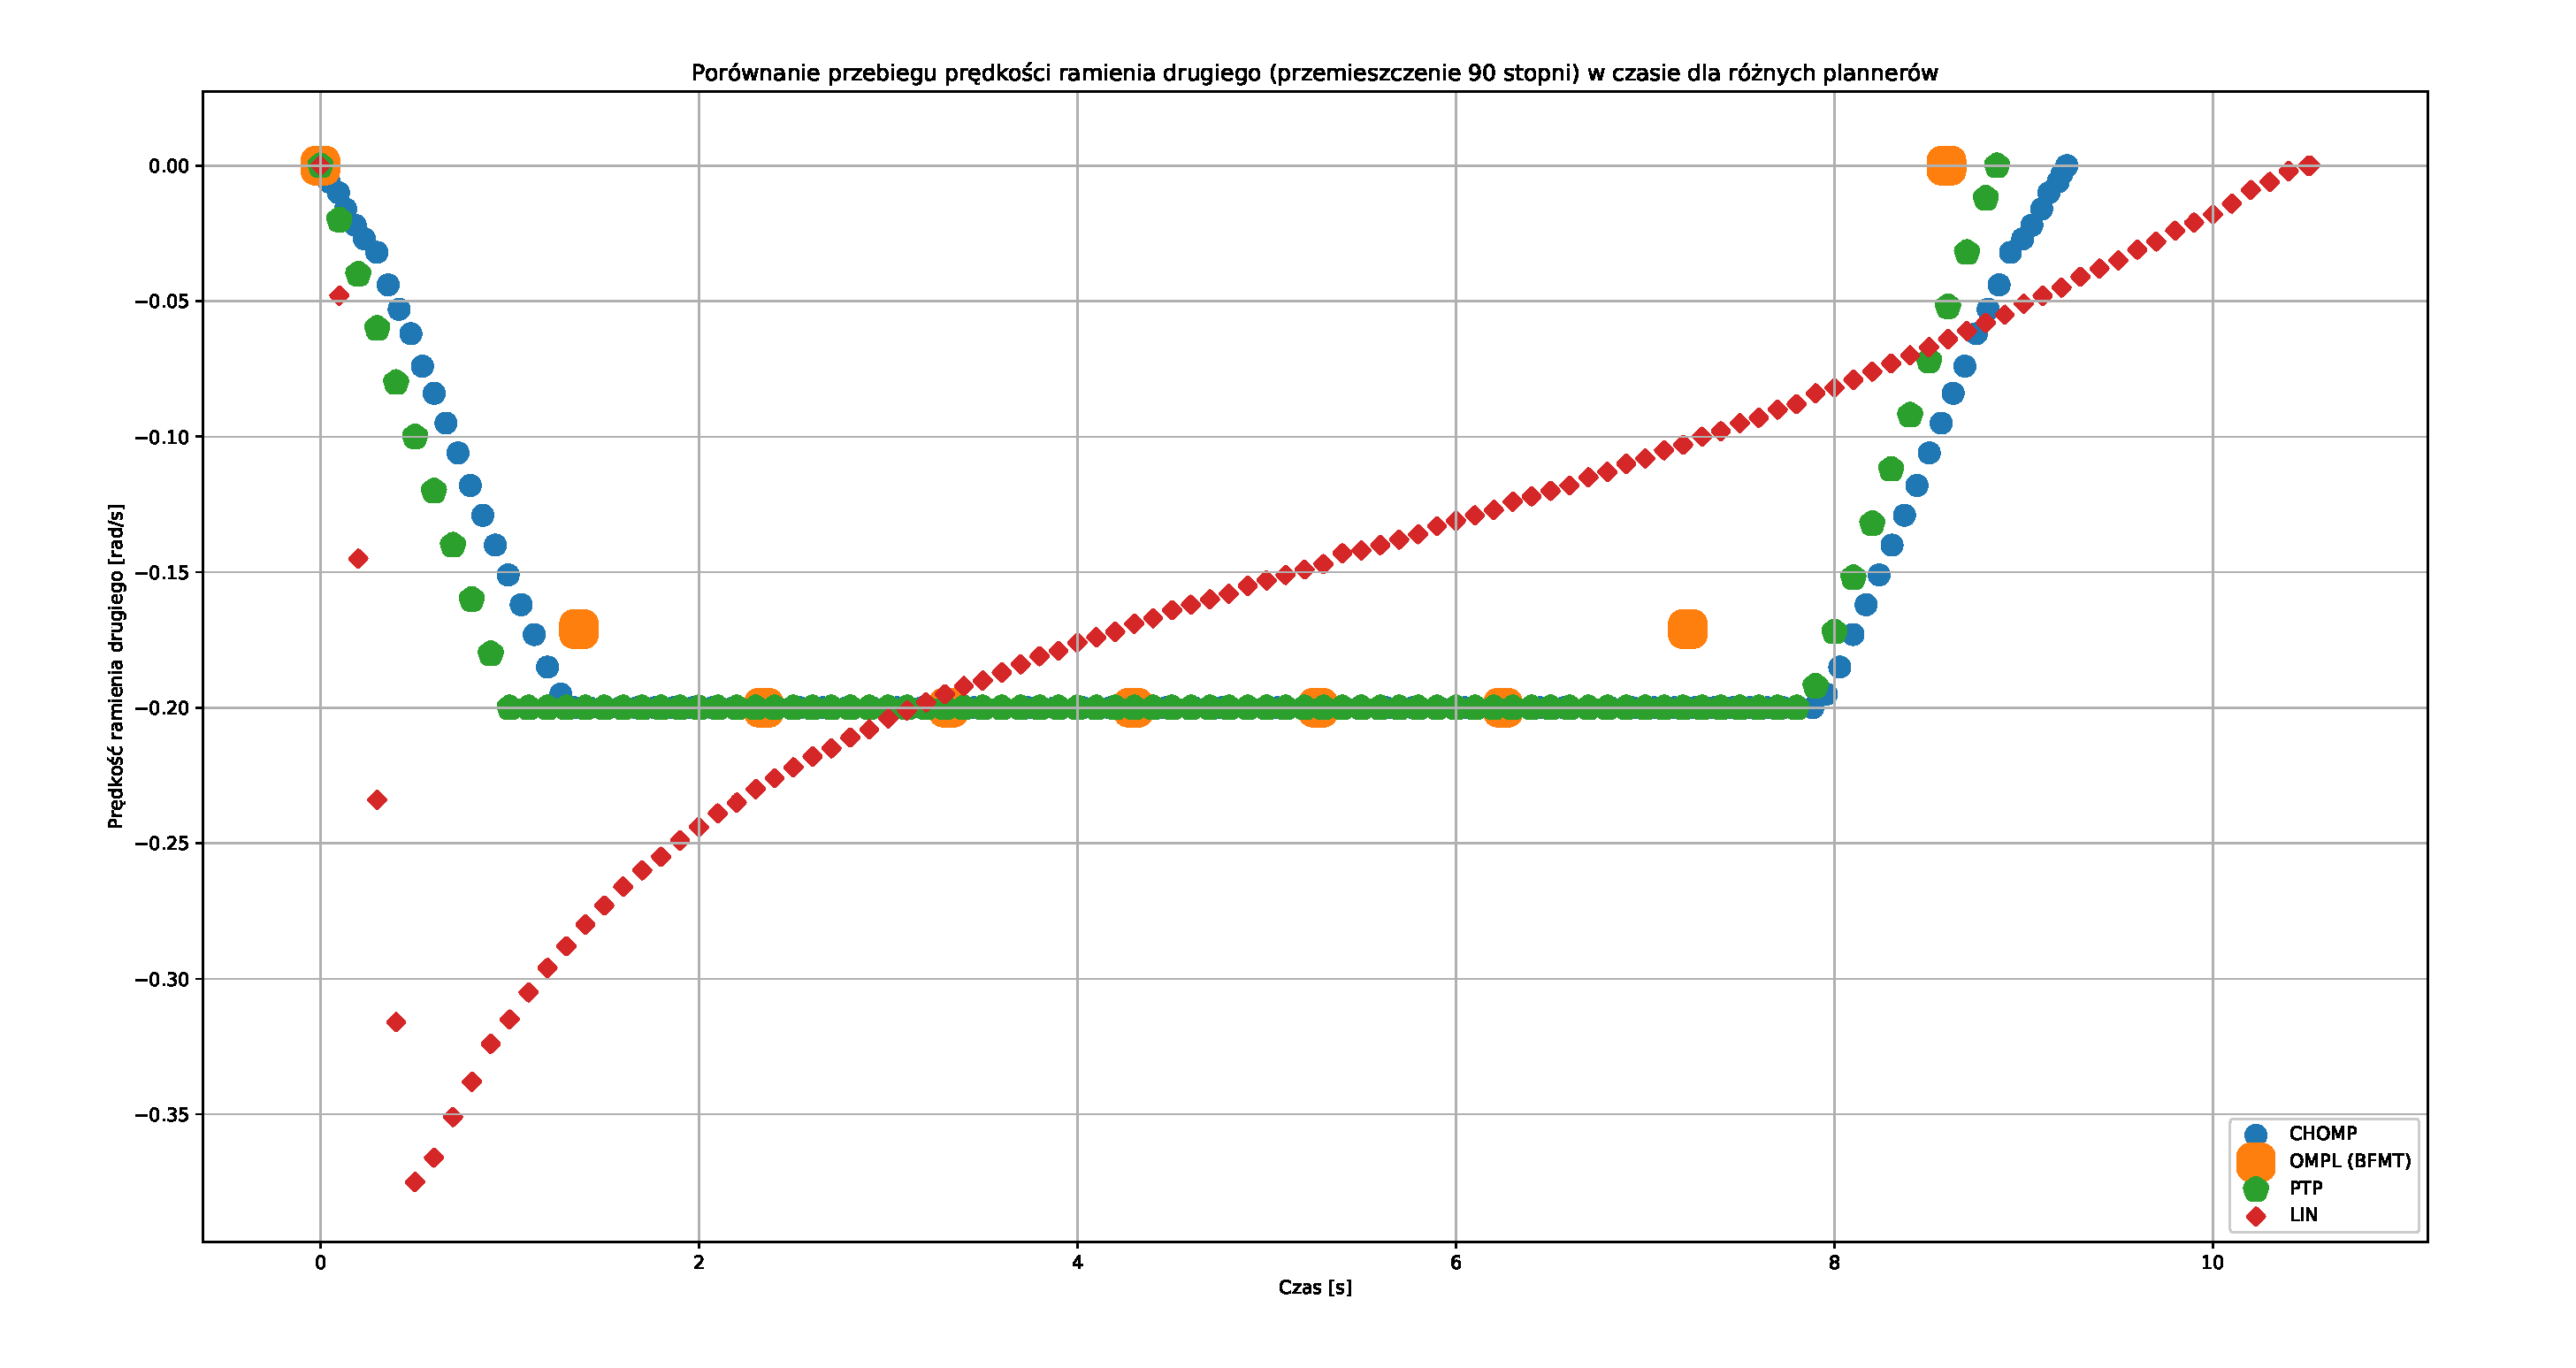
\includegraphics[width=1\linewidth]{{img/Figure_vel_90.eps}}
	\caption{Porównanie prędkości złącza ramienia drugiego w zależności od użytego plannera. \cite{plot_file}}
	\label{fig:32}
\end{figure}

Powyższy wykres \ref{fig:32} jednoznacznie odpowiada na poruszone w poprzednim akapicie kwestie. Mianowicie ilość generowanych przez plannery punktów nie jest stała - zależy od trasy. Wykres \ref{fig:32} uwypukla także charakterystyczny kształt realizacji trasy przez algorytm LIN.

Postanowiono także sprawdzić czy punkty generowane są w równych odstępach czasu, czy jednak nie. W tym celu wyznaczono minimalne i maksymalne różnice czasów między kolejnymi próbkami poprzedniego wykresu.

% Please add the following required packages to your document preamble:
% \usepackage{multirow}
% \usepackage[table,xcdraw]{xcolor}
% If you use beamer only pass "xcolor=table" option, i.e. \documentclass[xcolor=table]{beamer}
\begin{table}[H]
\centering
\caption{Porównanie różnic czasu między kolejnymi próbkami plannerów}
\label{tab:18}
\begin{tabular}{|c|c|c|c|
>{\columncolor[HTML]{C0C0C0}}c |ll}
\cline{1-5}
\cellcolor[HTML]{C0C0C0}L.p. & \cellcolor[HTML]{C0C0C0}{\color[HTML]{000000} \begin{tabular}[c]{@{}c@{}}Grupa \\ plannerów\end{tabular}} & \cellcolor[HTML]{C0C0C0}Planner & \cellcolor[HTML]{C0C0C0}\begin{tabular}[c]{@{}c@{}}Min. różnica czasu\\ między próbkami {[}s{]}\end{tabular} & \begin{tabular}[c]{@{}c@{}}Max. różnica czasu\\ między próbkami {[}s{]}\end{tabular} &  &  \\ \cline{1-5}
\cellcolor[HTML]{EFEFEF}1.   & CHOMP                                                                                                     & \cellcolor[HTML]{EFEFEF}CHOMP   & \cellcolor[HTML]{EFEFEF}0.01(9)                                                                              & \cellcolor[HTML]{EFEFEF}0.147                                                        &  &  \\ \cline{1-5}
\cellcolor[HTML]{C0C0C0}2.   & OMPL                                                                                                      & \cellcolor[HTML]{C0C0C0}BFMT    & \cellcolor[HTML]{C0C0C0}0.976                                                                                & 1.366                                                                                &  &  \\ \cline{1-5}
\cellcolor[HTML]{EFEFEF}3.   &                                                                                                           & \cellcolor[HTML]{EFEFEF}PTP     & \cellcolor[HTML]{EFEFEF}0.0(9)                                                                               & \cellcolor[HTML]{EFEFEF}0.1                                                          &  &  \\ \cline{1-1} \cline{3-5}
\cellcolor[HTML]{C0C0C0}4.   & \multirow{-2}{*}{\begin{tabular}[c]{@{}c@{}}Pilz Industrial \\ Motion Planner\end{tabular}}               & \cellcolor[HTML]{C0C0C0}LIN     & \cellcolor[HTML]{C0C0C0}0.0(9)                                                                               & 0.1                                                                                  &  &  \\ \cline{1-5}
\end{tabular}
\end{table}

Tabela obrazuje, iż największą zmienność w generowaniu próbek posiada algorytm CHOMP. Daje to istotną informację, że wraz ze zbliżaniem się do kluczowych elementów trasy, próbki zagęszczają się. Zmienność występuje także w przypadku grupy OMPL. Plannery Pilz Industrial raczej zdają się utrzymywać stały krok wyznaczania kolejnych punktów.

Dodatkowo według przeprowadzonych testów, ilość punktów jakie generują plannery (na podstawie OMPL FMT) nie zależy od ustawionej dokładności - goal bias. Za każdym razem zarówno prędkości jak i czasy przemieszczeń były identyczne. 

%Starając się wyczerpać tematykę zaplanowanych punktów i prędkości złącz postanowiono jeszcze zestawić przebiegi wszystkich złącz, niemniej w sytuacji omijania przeszkody. Tematyka ta zostanie dokładnie omówiona w kolejnych sekcjach, niemniej celem niniejszego eksperymentu było sprawdzenie, jak zachowuje się algorytm w przypadku ruchu złożonego. Poniżej zaprezentowano wykres przedstawiający prędkości wszystkich osi - wykres \ref{fig:33}.

\begin{figure}[H]
	\centering
	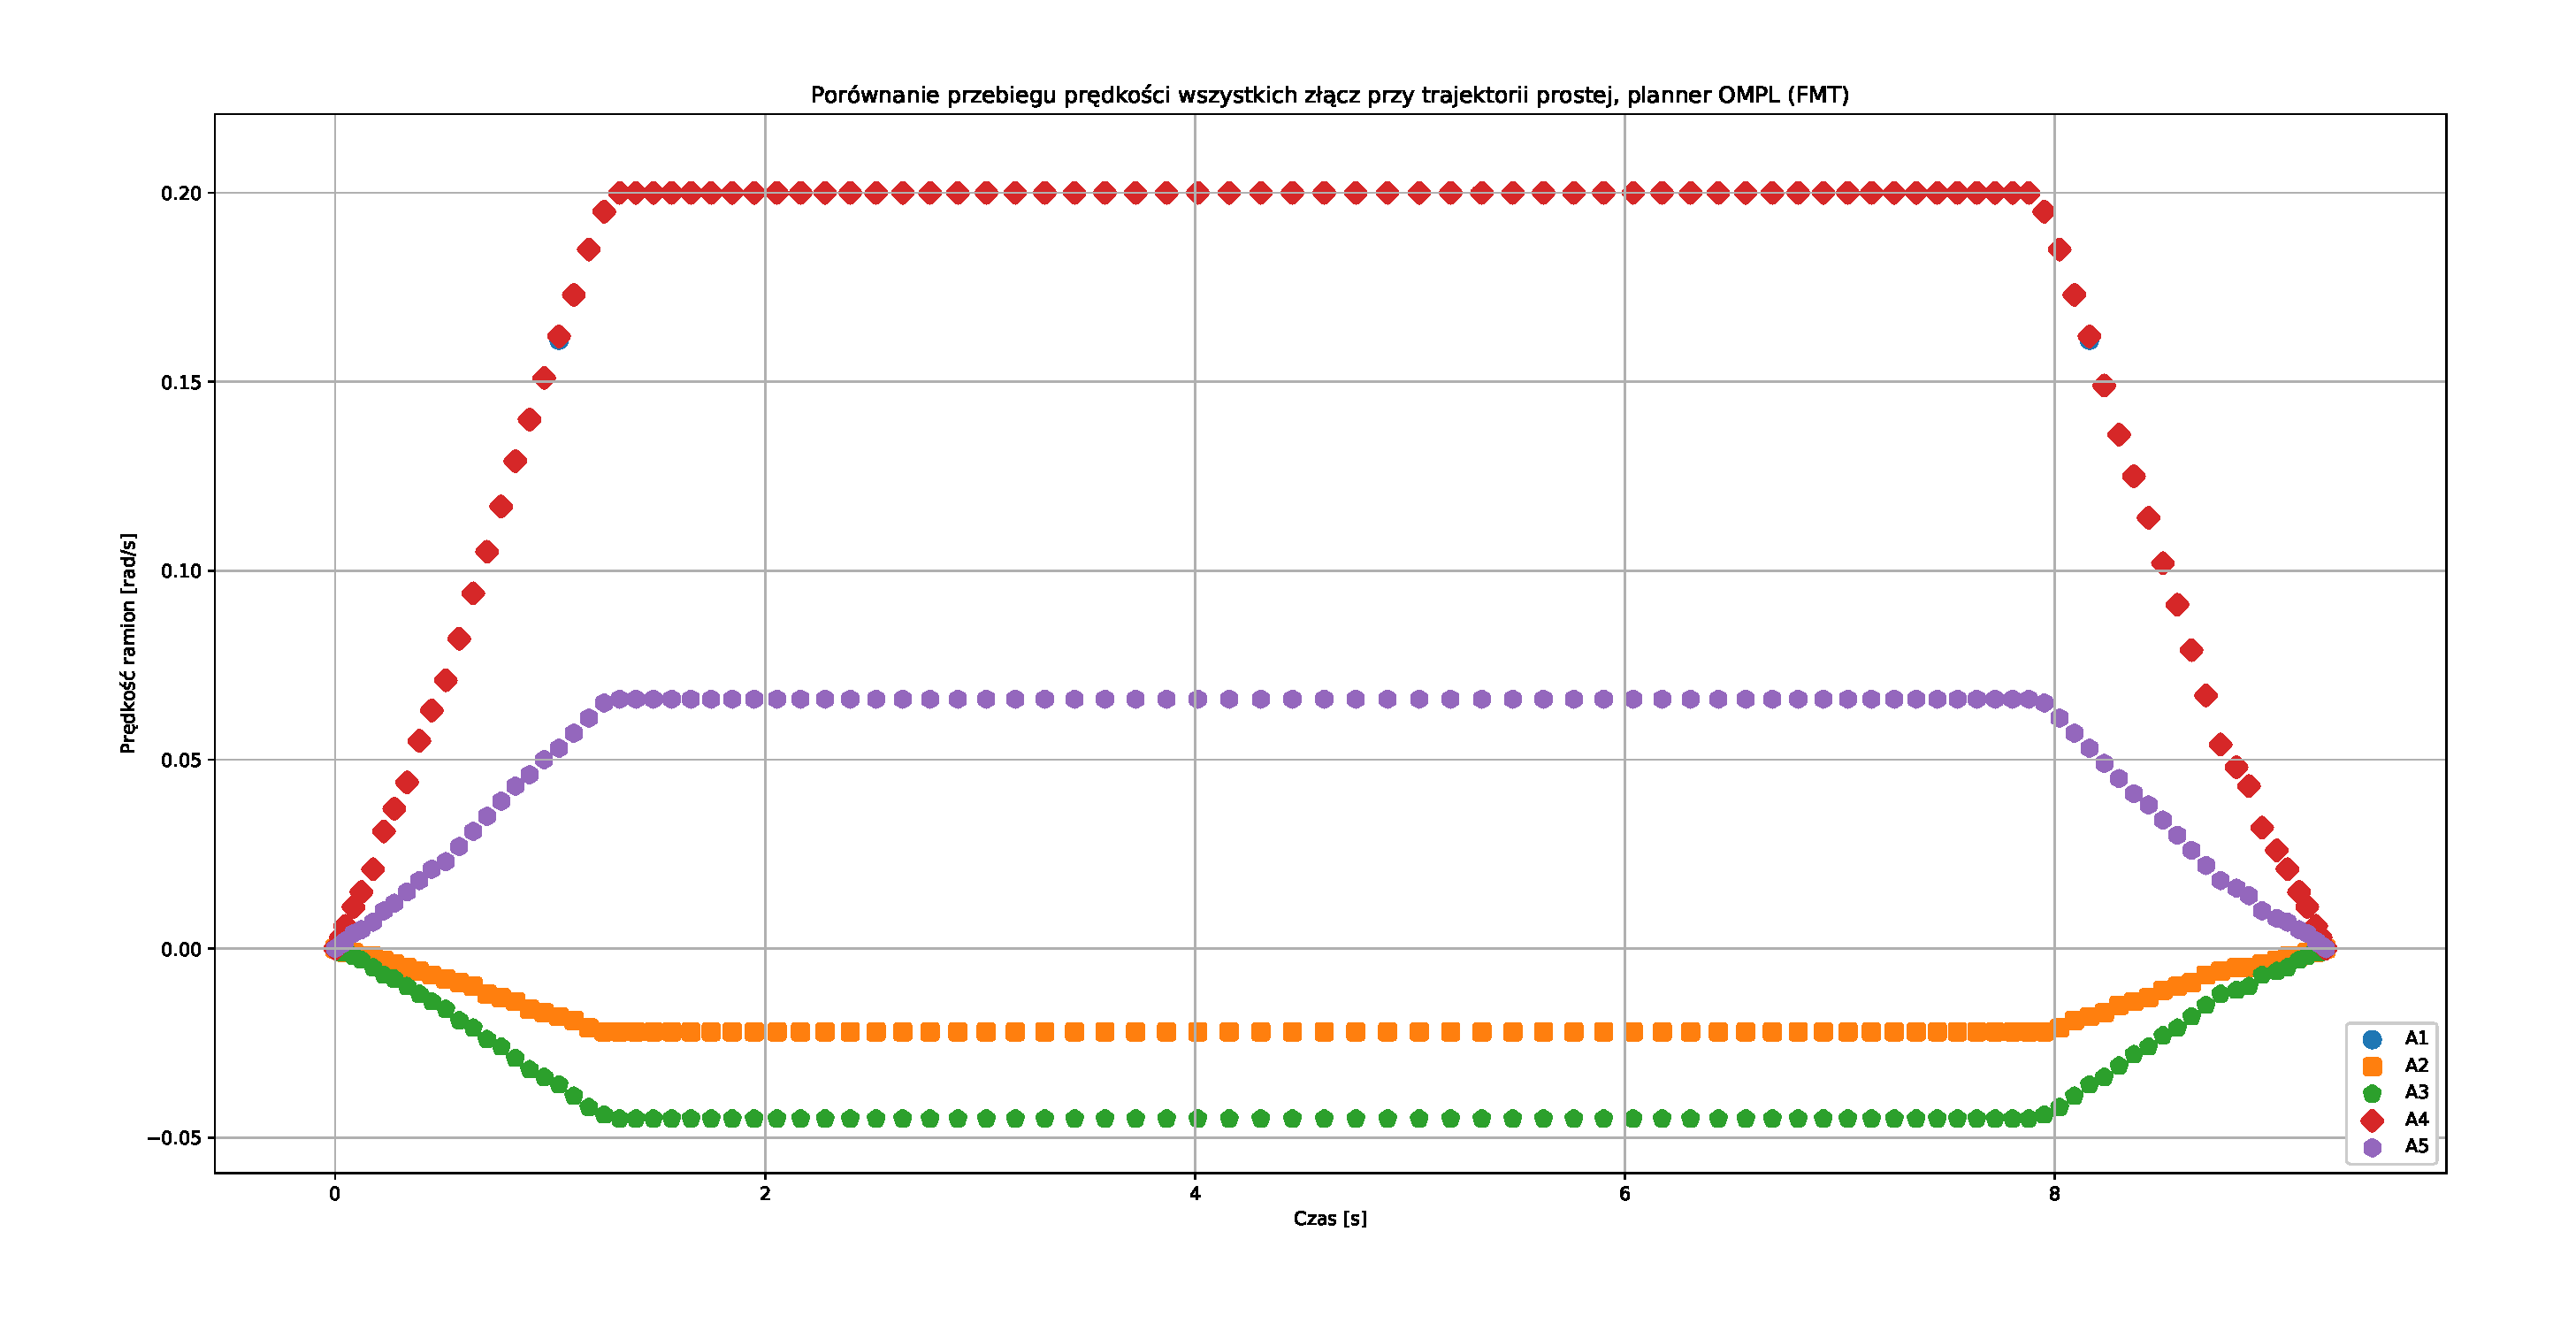
\includegraphics[width=1\linewidth]{{img/Figure_synchro.eps}}
	\caption{Porównanie prędkości wszystkich złącz przy omijaniu przeszkody dla plannera OMPL FMT. \cite{plot_file}}
	\label{fig:33}
\end{figure}


Powyższy wykres ilustruje dwie kwestie. Pierwszą rzeczą jest skalowanie prędkości złącz. Osie są względem siebie synchronizowane, tak by wszystkie zakończyły swój ruch dokładnie w tym samym czasie. Co ciekawe skalowanie prędkości poszczególnych złącz następuje w przypadku wszystkich plannerów. Nie ma tutaj także znaczenia czy następuje omijanie przeszkody, czy normalne przemieszczenie.

Druga kwestia jaką prezentuje wykres \ref{fig:33} to zagęszczanie próbek, o którym poprzednio wspominano. Na wykresie widać to doskonale.


 \newpage
 
\subsection{Omijanie przeszkód}

Niniejszy podrozdział poświęcono kwestii omijania przeszkód. Przetestowano zatem czy dany algorytm jest w stanie realizować takie zadanie, a także w jaki sposób to czyni. 

Rviz umożliwia użytkownikowi dodanie do scenografii otaczającej robota dodatkowych obiektów, które manipulator może traktować jako przedmioty kolizyjne. W tym celu zaproponowano zatem prostą sytuację, w której to robota ma przemieścić swoje ramię w płaszczyźnie pionowej, z tym zastrzeżeniem iż na trasie tej umieszczono obiekt. Całość prezentowała się tak jak poniżej - rysunek \ref{fig:34}. 

Przygotowana sytuacja była dosyć prosta, niemniej wymagała od plannera ominięcia dołączonego prostopadłościanu.  Poniższa tabela prezentuje zestawienie algorytmów ze względu na te które potrafiły i nie potrafiły znaleźć trasy.

\begin{figure}[H]
	\centering
	\includegraphics[width=1\linewidth]{{img/Bild_rviz_scene.png}}
	\caption{\centering Przygotowany scenariusz omijania przeszkody w programie Rviz. \cite{own}, \cite{oak}}
	\label{fig:34}
\end{figure}


W czasie eksperymentów wyszło, iż zarówno plannery grupy CHOMP oraz Pilz Industrial nie są w stanie omijać przeszkód. Jest to bardzo istotne przy ewentualnej chęci ich stosowania. Zatem eksperymenty przeprowadzano jedynie na grupie algorytmów OMPL. W poniższej tabeli zestawiono otrzymane rezultaty. Przy czym te plannery, które nie zostały w niej zawarte nie były  w stanie zaplanować trasy przy narzuconych warunkach. 

Ustawienia były w każdym przypadku domyślne. Maksymalna ilość prób jaką miały do wykorzystania algorytmy ustawiono na 10, natomiast czas planowania - 10 sekund. Za każdym razem dokonywano 10 prób. Długości tras jakie zestawiono w poniższej tabeli \ref{tab:7} odnoszą się do sumarycznego przemieszczenia wszystkich złącz na całej trasie. Natomiast czasy oznaczają ustalony teoretyczny czas potrzebny na realizację trajektorii.

% Please add the following required packages to your document preamble:
% \usepackage[table,xcdraw]{xcolor}
% If you use beamer only pass "xcolor=table" option, i.e. \documentclass[xcolor=table]{beamer}
\begin{table}[H]
\centering
\caption{Zestawienie długości i czasów zaplanowanych tras przy omijaniu przeszkody}
\label{tab:7}
\begin{tabular}{|c|c|c|c|c|c|c|c|}
\hline
\rowcolor[HTML]{C0C0C0} 
Lp  & Planner  & \begin{tabular}[c]{@{}c@{}}Min. wy. \\ trasa \\ {[}rad{]}\end{tabular} & \cellcolor[HTML]{C0C0C0}\begin{tabular}[c]{@{}c@{}}Max. wy.\\  trasa \\ {[}rad{]}\end{tabular} & \begin{tabular}[c]{@{}c@{}}Śr. wy.\\ trasa 10 \\ pr. {[}rad{]}\end{tabular} & \cellcolor[HTML]{C0C0C0}\begin{tabular}[c]{@{}c@{}}Min. wy.\\ czas {[}s{]}\end{tabular} & \cellcolor[HTML]{C0C0C0}\begin{tabular}[c]{@{}c@{}}Max. wy.\\  czas {[}s{]}\end{tabular} & \cellcolor[HTML]{C0C0C0}\begin{tabular}[c]{@{}c@{}}Śr. czas \\ 10 pr. \\ {[}s{]}\end{tabular} \\ \hline
\rowcolor[HTML]{9AFF99} 
1.  & BFMT     & 7.791                                                                  & 10.262                                                                                         & 9.228                                                                       & 5.248                                                                                   & 5.965                                                                                    & 5.494                                                                                         \\ \hline
\rowcolor[HTML]{FFCCC9} 
2.  & BKPIECE  & 15.008                                                                 & 262.628                                                                                        & 158.649                                                                     & 6.767                                                                                   & 31.546                                                                                   & 24.905                                                                                        \\ \hline
\rowcolor[HTML]{EFEFEF} 
3.  & BiEST    & 9.698                                                                  & 38.919                                                                                         & 21.638                                                                      & 5.775                                                                                   & 17.095                                                                                   & 9.148                                                                                         \\ \hline
\rowcolor[HTML]{C0C0C0} 
4.  & BiTRRT   & 7.396                                                                  & 149.674                                                                                        & 23.704                                                                      & 4.607                                                                                   & 24.939                                                                                   & 7.577                                                                                         \\ \hline
\rowcolor[HTML]{FFCCC9} 
5.  & EST      & 10.210                                                                 & 66.61                                                                                          & 33.300                                                                      & 6.380                                                                                   & 20.419                                                                                   & 11.958                                                                                        \\ \hline
\rowcolor[HTML]{C0C0C0} 
6.  & FMT      & 7.800                                                                  & 93.849                                                                                         & 18.560                                                                      & 4.704                                                                                   & 16.837                                                                                   & 6.697                                                                                         \\ \hline
\rowcolor[HTML]{EFEFEF} 
7.  & KPIECE   & 10.066                                                                 & 54.170                                                                                         & 25.301                                                                      & 5.708                                                                                   & 19.966                                                                                   & 10.594                                                                                        \\ \hline
\rowcolor[HTML]{C0C0C0} 
8.  & PDST     & 8.374                                                                  & 107.111                                                                                        & 28.119                                                                      & 5.305                                                                                   & 20.763                                                                                   & 8.865                                                                                         \\ \hline
\rowcolor[HTML]{EFEFEF} 
9.  & PRM      & 10.701                                                                 & 34.114                                                                                         & 19.477                                                                      & 6.402                                                                                   & 13.292                                                                                   & 9.314                                                                                         \\ \hline
\rowcolor[HTML]{C0C0C0} 
10. & PRMstar  & 8.981                                                                  & 13.459                                                                                         & 11.366                                                                      & 5.271                                                                                   & 7.479                                                                                    & 6.357                                                                                         \\ \hline
\rowcolor[HTML]{EFEFEF} 
11. & ProjEST  & 11.252                                                                 & 50.101                                                                                         & 25.690                                                                      & 5.845                                                                                   & 18.427                                                                                   & 10.314                                                                                        \\ \hline
\rowcolor[HTML]{C0C0C0} 
12. & RRTCon.  & 12.593                                                                 & 29.065                                                                                         & 20.996                                                                      & 6.664                                                                                   & 12.848                                                                                   & 9.635                                                                                         \\ \hline
\rowcolor[HTML]{EFEFEF} 
13. & RRT      & 8.644                                                                  & 21.57                                                                                          & 12.807                                                                      & 4.842                                                                                   & 8.85                                                                                     & 6.182                                                                                         \\ \hline
\rowcolor[HTML]{9AFF99} 
14. & RRTstar  & 7.823                                                                  & 19.641                                                                                         & 10.944                                                                      & 4.555                                                                                   & 8.355                                                                                    & 5.914                                                                                         \\ \hline
\rowcolor[HTML]{EFEFEF} 
15. & SBL      & 9.764                                                                  & 51.741                                                                                         & 23.404                                                                      & 6.326                                                                                   & 16.221                                                                                   & 9.087                                                                                         \\ \hline
\rowcolor[HTML]{C0C0C0} 
16. & SPARS    & 8.754                                                                  & 22.987                                                                                         & 14.749                                                                      & 5.560                                                                                   & 11.671                                                                                   & 7.808                                                                                         \\ \hline
\rowcolor[HTML]{EFEFEF} 
17. & SPARStwo & 10.490                                                                 & 24.671                                                                                         & 17.792                                                                      & 6.722                                                                                   & 11.141                                                                                   & 8.392                                                                                         \\ \hline
\rowcolor[HTML]{C0C0C0} 
18. & STRIDE   & 8.957                                                                  & 54.592                                                                                         & 23.254                                                                      & 5.794                                                                                   & 13.063                                                                                   & 8.596                                                                                         \\ \hline
\rowcolor[HTML]{9AFF99} 
19. & TRRT     & 8.032                                                                  & 10.96                                                                                          & 9.181                                                                       & 5.024                                                                                   & 6.133                                                                                    & 5.433                                                                                         \\ \hline
\end{tabular}
\end{table}

Jak można zauważyć na załączonej tabeli, najgorszy okazał się planner BKPIECE. Trasy które za każdym razem wyznaczał były czasem absurdalnie długie. Niemniej podobnie jak w poprzednich testach, tak i obecnie bardzo pozytywnie wyszedł algorytm TRRT. 

Ciekawy jest również sam fakt występujących różnic za każdą próbą planowania. Wyznaczona trasa za każdym razem jest inna. Nie jest to proces jednoznacznie deterministyczny. 

Poniżej zaprezentowano wykres przestrzenny, na którym zaprezentowano kilka zaproponowanych przez plannerów tras, tak by zobrazować problem różności trajektorii. Na wykresie zaprezentowano także szkielet obiektu stanowiącego przeszkodę - rysunek \ref{fig:35}. 

 \begin{figure}[H]
	\centering
	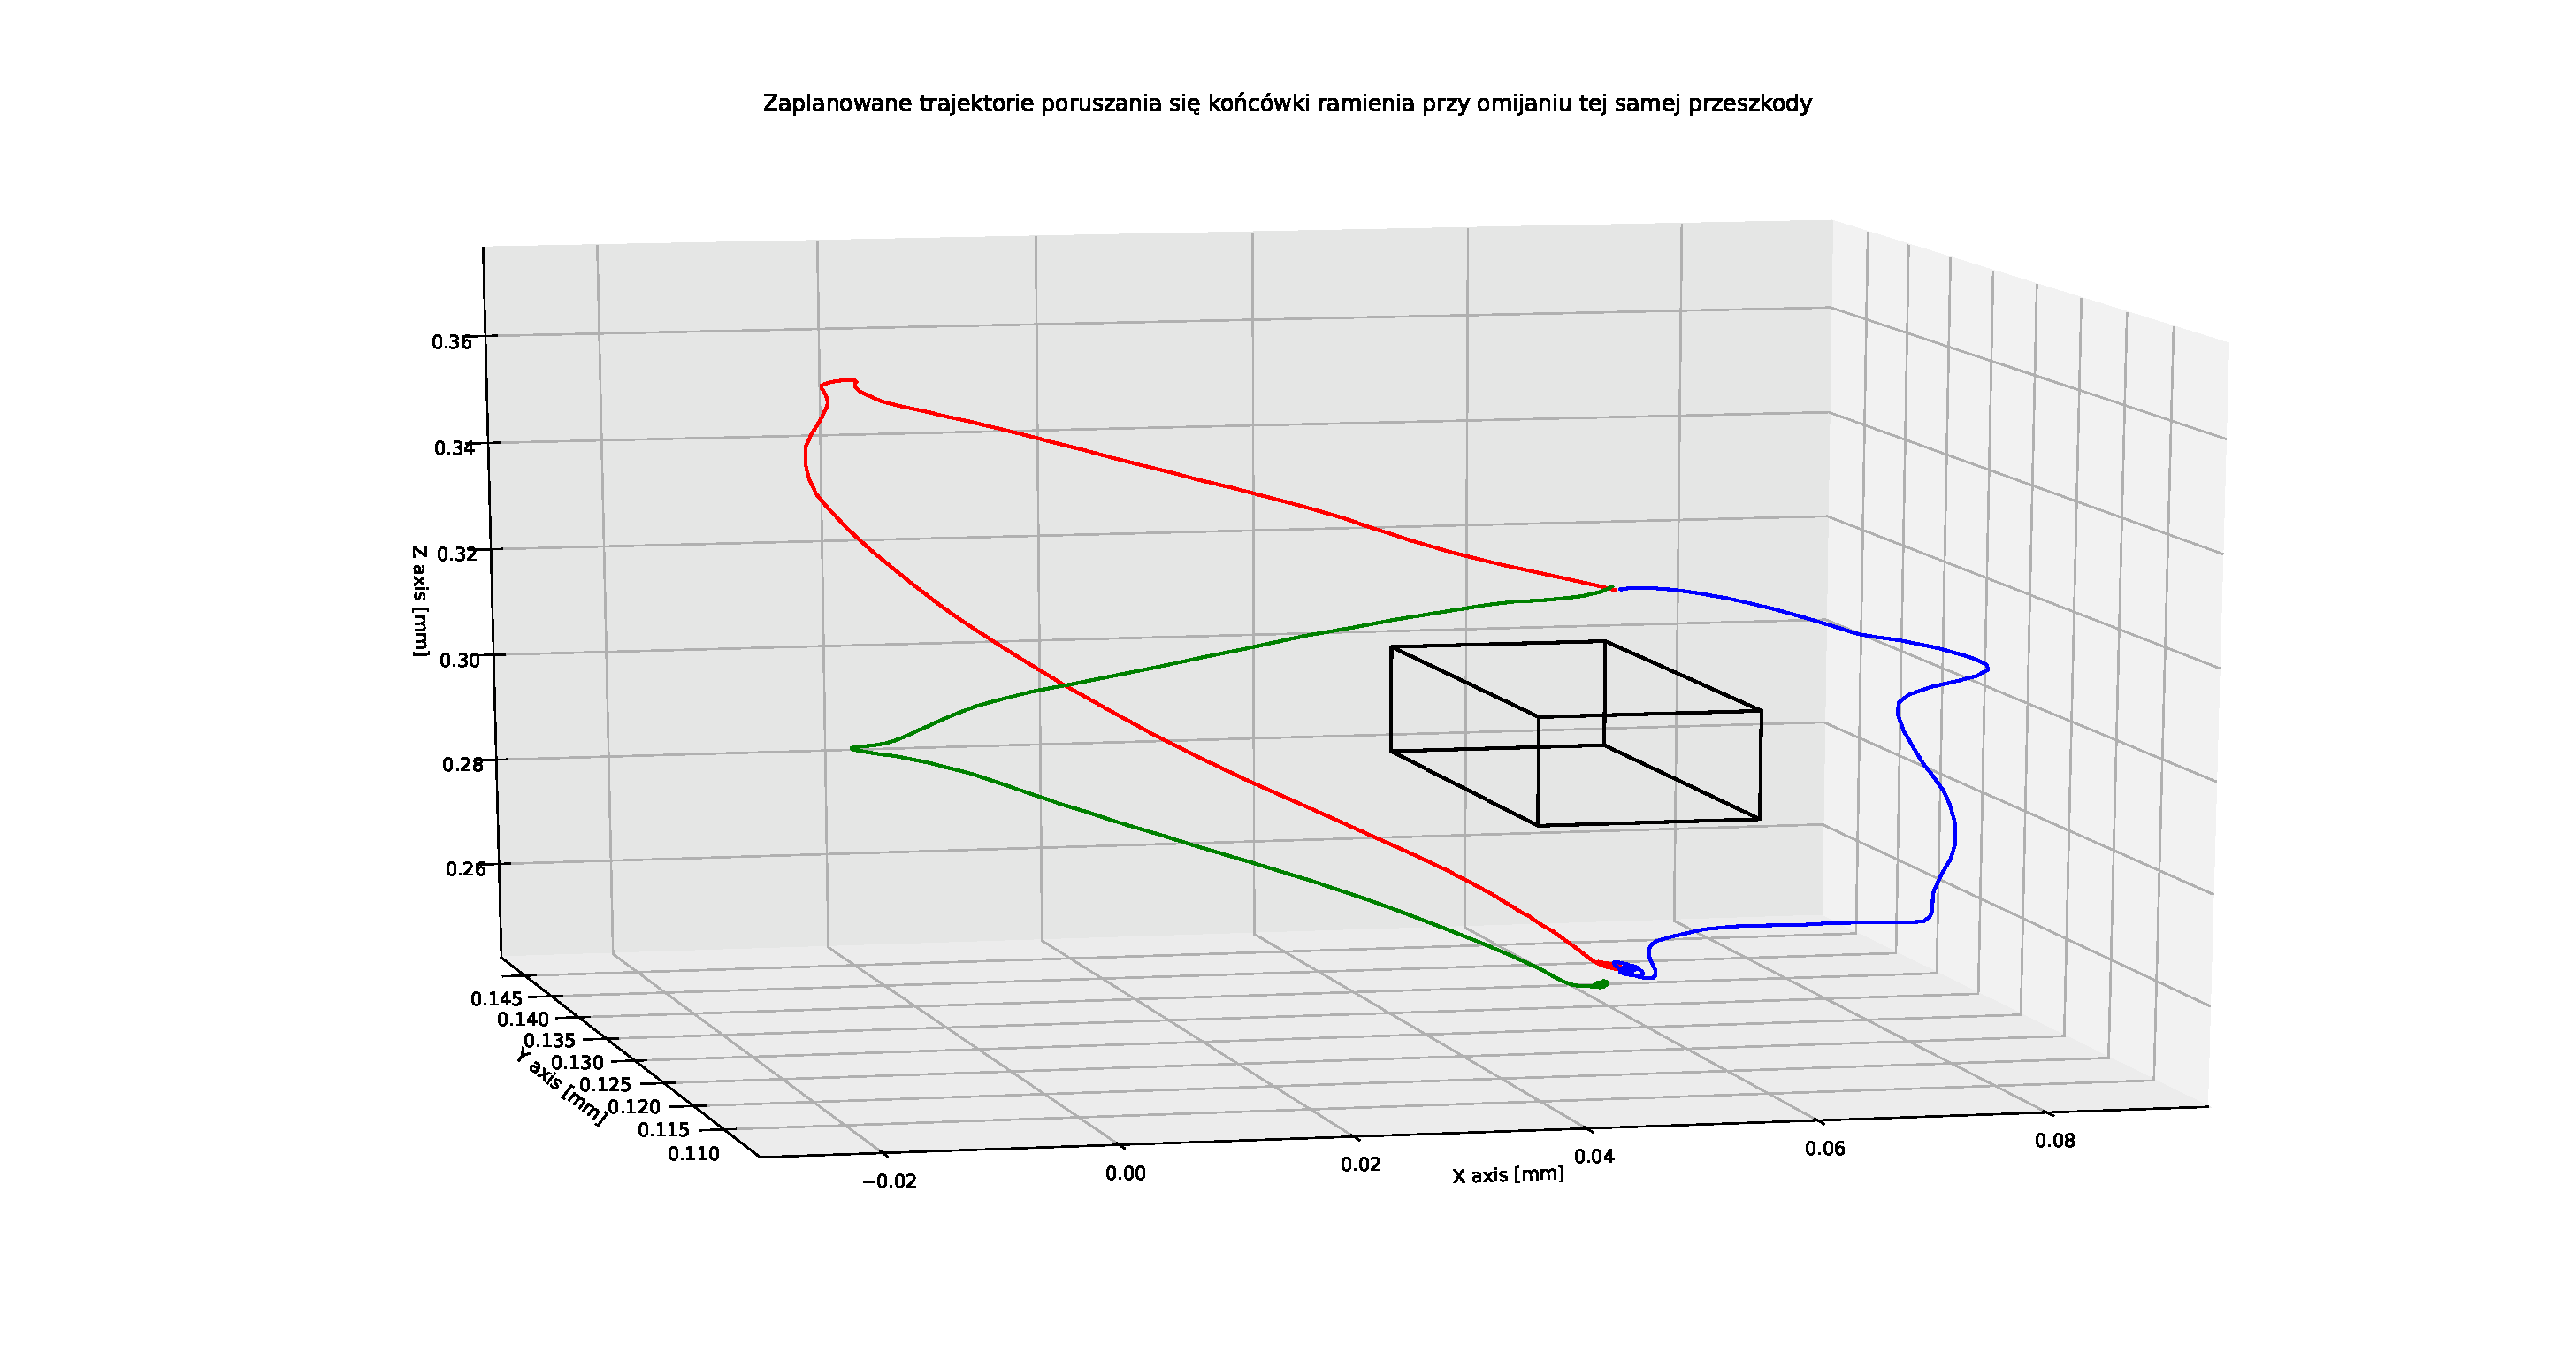
\includegraphics[width=1\linewidth]{{img/Figure_omitt.eps}}
	\caption{Zaplanowane trajektorie poruszania się końcówki ramienia przy omijaniu tej samej przeszkody. \cite{plot_file}}
	\label{fig:35}
\end{figure}

Podsumowując nieco zaprezentowane w tym podrozdziale eksperymenty, można powiedzieć, iż proces omijania przez manipulator nawet prostej przeszkody, nie jest zagadnieniem oczywistym. Plannery, które do tej pory uznawano za bardzo skuteczne (PTP, LIN, CHOMP) okazały się w ogóle nie realizować tego problemu. Niemniej pozytywną kwestią jest, iż istnieją algorytmy wchodzące w skład grupy OMPL, które bardzo dobrze radzą sobie z tym zagadnieniem, w konsekwencji czego, nadal MoveIt może służyć jako kontroler, także przy tego typu zastosowaniach.


\subsection{Trajektorie złożone}

Do tej pory testowano i porównywano ze sobą plannery jakie udostępniał MoveIt. Niezależnie od tego jakie trasy algorytmy te zaproponowały, były to trajektorie teoretyczne, po jakich miało się poruszać ramię robota. Niemniej w rzeczywistości robot nie podąża jednoznacznie za nimi, ze względu na ograniczenia konstrukcyjne i ogólnie fizykę. Toteż kolejna sekcja eksperymentów poświęcona została porównywaniu zachowań robota w środowisku symulacyjnym Gazebo oraz fizycznego urządzenia. 

Roboty przemysłowe są przystosowane do wykonywania często dwóch typów zadań. Pierwszym z nich jest klasyczne zadanie przenoszenia obiektów, tzw. zadanie $pick$ $and$ $place$.
Natomiast drugi typ zadań, jest związany ze sterowaniem robota w układzie kartezjańskim, tj. w sytuacji kiedy to końcówka robocza urządzenia utrzymuje np. stałą wysokość i orientację. Zadania takie są bardzo istotne np. w momencie spawania bądź nanoszenia kleju gdzie należy przesuwać ramię w jednej ustalonej płaszczyźnie, jednocześnie stale utrzymując zadaną odległość od obiektu.

Zaczynając od pierwszego ze wspomnianych zadań, postanowiono przygotować odpowiedni eksperyment. Jako, iż w oprogramowaniu Rviz nie jest możliwe wyznaczanie trajektorii złożonych, toteż napisano w tym celu węzeł ROS (język Python), który sekwencyjnie realizuje konieczną trasę. Robot nie został wyposażony w tor wizyjny, przez co trasę dobrano eksperymentalnie, docelowo powinien to realizować algorytm korzystający z zainstalowanych na urządzeniu kamer. \cite{PaP_file}

Jak wspominano w rozdziale poświęconym modelowi robota w Gazebo - \ref{sub:ModelGazebo}, do symulacji dodano niewielki obiekt, tak by urządzenie mogło go chwycić. Istotne było nadanie obiektowi należytych parametrów - takich jak masa, inercja oraz sprężystość. Bez nich robot nie był w stanie go przemieścić, gdyż albo był dla niego za ciężki, albo też nie dawał się złapać, ze względu na zbyt twardą powierzchnię. Parametry te jednocześnie nie powinny być także zbyt małe, gdyż wówczas manipulator nie był w stanie upuścić przedmiotu po przemieszczeniu. 

 \begin{figure}[H]
	\centering
	\includegraphics[width=1\linewidth]{{img/Bild_seife.png}}
	\caption{\centering Symulowany w Gazebo robot trzymający transportowany obiekt. \cite{own}, \cite{oak}}
	\label{fig:38}
\end{figure}

Uruchamiając sekwencję zbierano kolejne punkty w jakich znajdowało się urządzenie, tak by móc je później porównać ze sobą. Eksperyment przeprowadzono jednocześnie na symulacji oraz na faktycznym urządzeniu. W eksperymentach na fizycznym robocie wykorzystano pudełko zapałek, jako obiekt do transportu. W załącznikach do niniejszej pracy zamieszczono wideo, przedstawiające rzeczywistego robota realizującego opisywane zadanie. \cite{movie_file}

Uzyskanie punktów w przestrzeni kartezjańskiej dla rozwiązywanego zadania wymagało liczenia kinematyki prostej. Z wykorzystaniem ROS problem ten nie jest trudny do zrealizowania, gdyż udostępnia on funkcje, które na podstawie modelu robota (plik .urdf), przeliczają pozycje złączowe na punkty w przestrzeni.

Przeprowadzając eksperymenty zebrano pomiary, na podstawie których opracowano poniższy wykres - \ref{fig:36}

 \begin{figure}[H]
	\centering
	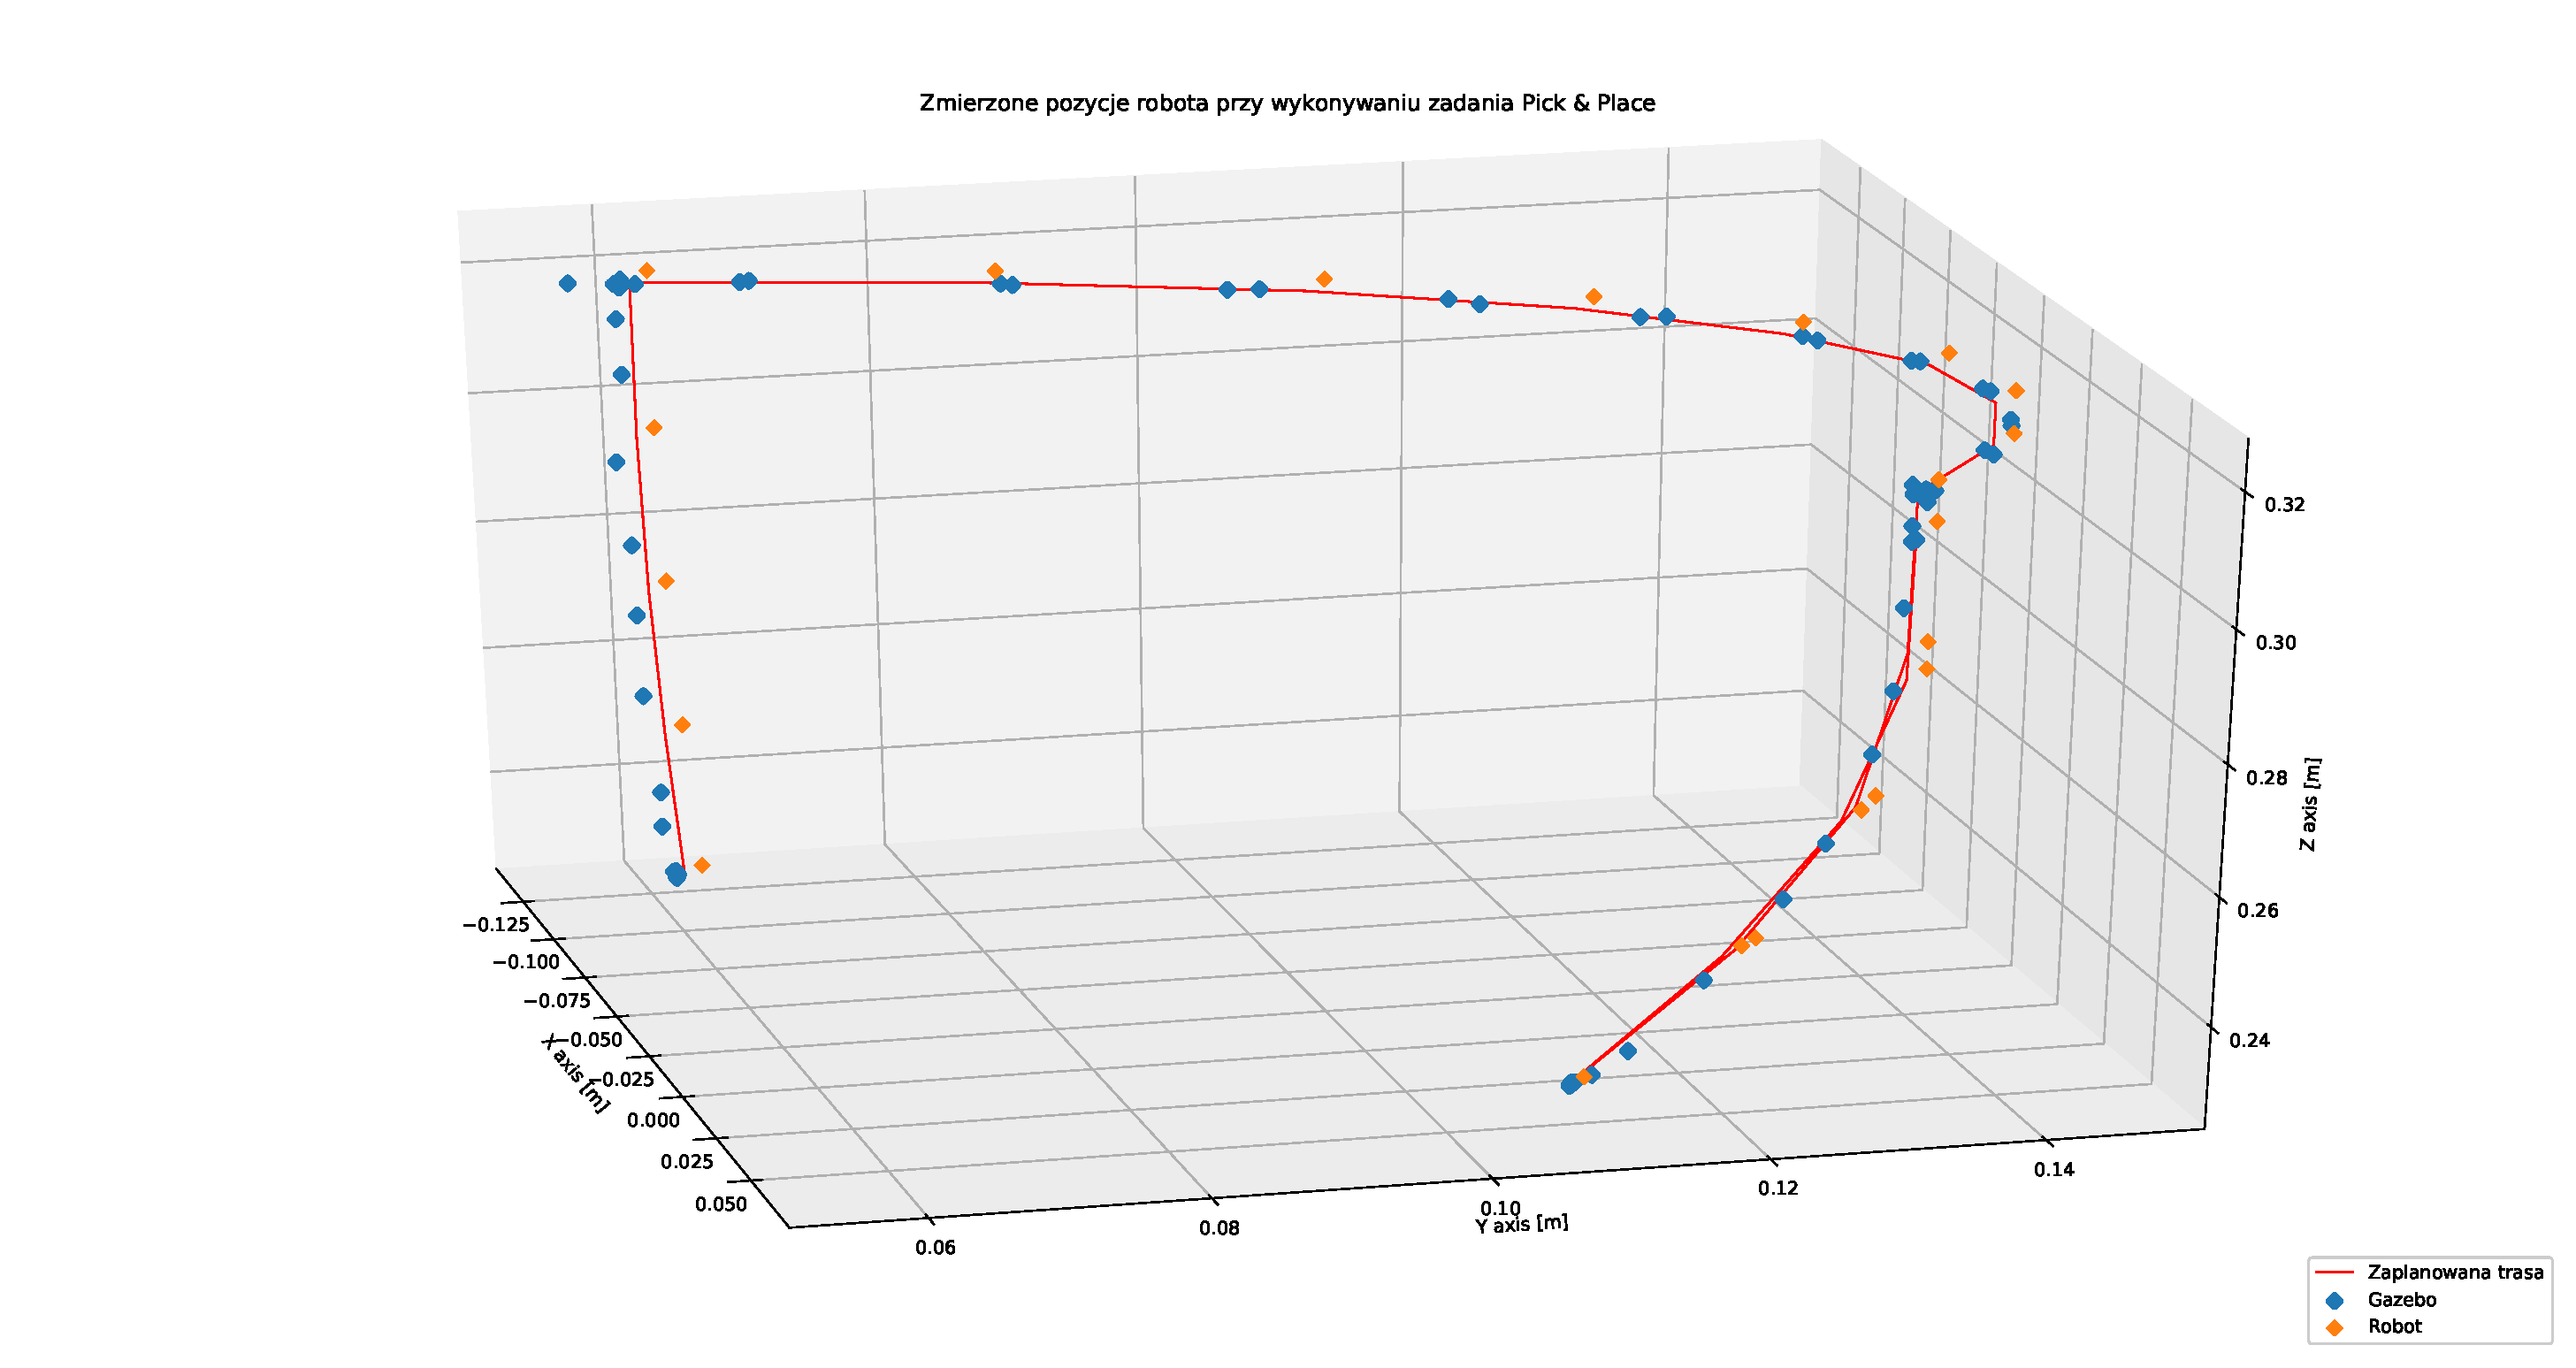
\includegraphics[width=1\linewidth]{{img/Figure_pap_com.eps}}
	\caption{Zmierzone pozycje robota przy wykonywaniu zadania Pick and Place. \cite{own}}
	\label{fig:36}
\end{figure}

Na podstawie zebranych punktów postanowiono policzyć różnicę między zaplanowaną trasą a faktycznymi punktami. Zatem kolejny raz posłużono się językiem Python. Napisano skrypt interpolujący punkty zaplanowanej trasy. W kolejnym kroku dla każdego pomiaru pochodzącego od Gazebo oraz z fizycznego robota policzono najkrótszy dystans do zinterplowanej krzywej. W ten sposób policzono minimalne odchylenie, maksymalne, a także wartość średnią.

% Please add the following required packages to your document preamble:
% \usepackage[table,xcdraw]{xcolor}
% If you use beamer only pass "xcolor=table" option, i.e. \documentclass[xcolor=table]{beamer}
\begin{table}[H]
\centering
\caption{Porównanie odchyleń zmierzonych punktów robota w czasie wykonywania zadania Pick \& Place}
\label{tab:8}
\begin{tabular}{|c|c|c|c|c|}
\hline
\rowcolor[HTML]{C0C0C0} 
Lp & Model  & \begin{tabular}[c]{@{}c@{}}Min.\\ odchyłka\\ {[}m{]}\end{tabular} & \cellcolor[HTML]{C0C0C0}\begin{tabular}[c]{@{}c@{}}Max.\\ odchyłka\\ {[}m{]}\end{tabular} & \begin{tabular}[c]{@{}c@{}}Śr.\\ odchyłka\\ {[}m{]}\end{tabular} \\ \hline
\rowcolor[HTML]{9AFF99} 
1. & Gazebo & 0.00010                                                           & 0.00396                                                                                   & 0.00066                                                          \\ \hline
\rowcolor[HTML]{FFCCC9} 
2. & Robot  & 0.00059                                                           & 0.00469                                                                                   & 0.00243                                                          \\ \hline
\end{tabular}
\end{table}


Teoretycznie model w Gazebo wypada w tym zestawieniu lepiej. Niemniej należy pamiętać, iż Gazebo realizuje ruch osi w oparciu o regulator PID i to w dużej mierze od jego nastaw zależy jak dobrze symulacją będzie podążała za zaplanowaną trasą. Natomiast faktyczny robot jest wyposażony w silniki krokowe. Zatem sterowanie nimi polega na podaniu ilości kroków jakie mają wykonać. Na tej podstawie wszystkie występujące zaokrąglenia do całkowitej liczby impulsów wprowadzają przekłamania. Kolejnym powodem dla którego faktyczny robot odznaczył się gorszą dokładnością jest występująca na złączą ramienia głównego nieliniowość. Wspominano już o tym w pracy inżynierskiej, iż sposób ukształtowania napędu ramienia głównego wprowadza pewne nieliniowości.


Drugi eksperyment dotyczył ruchu we współrzędnych kartezjańskich. Okazuje się, iż MoveIt również udostępnia tąże funkcjonalność. Podobnie jak to było wcześniej - nie można tego dokonać bezpośrednio z poziomu Rviza, toteż należało w tym celu napisać odpowiedni węzeł ROS. 

 \begin{figure}[H]
	\centering
	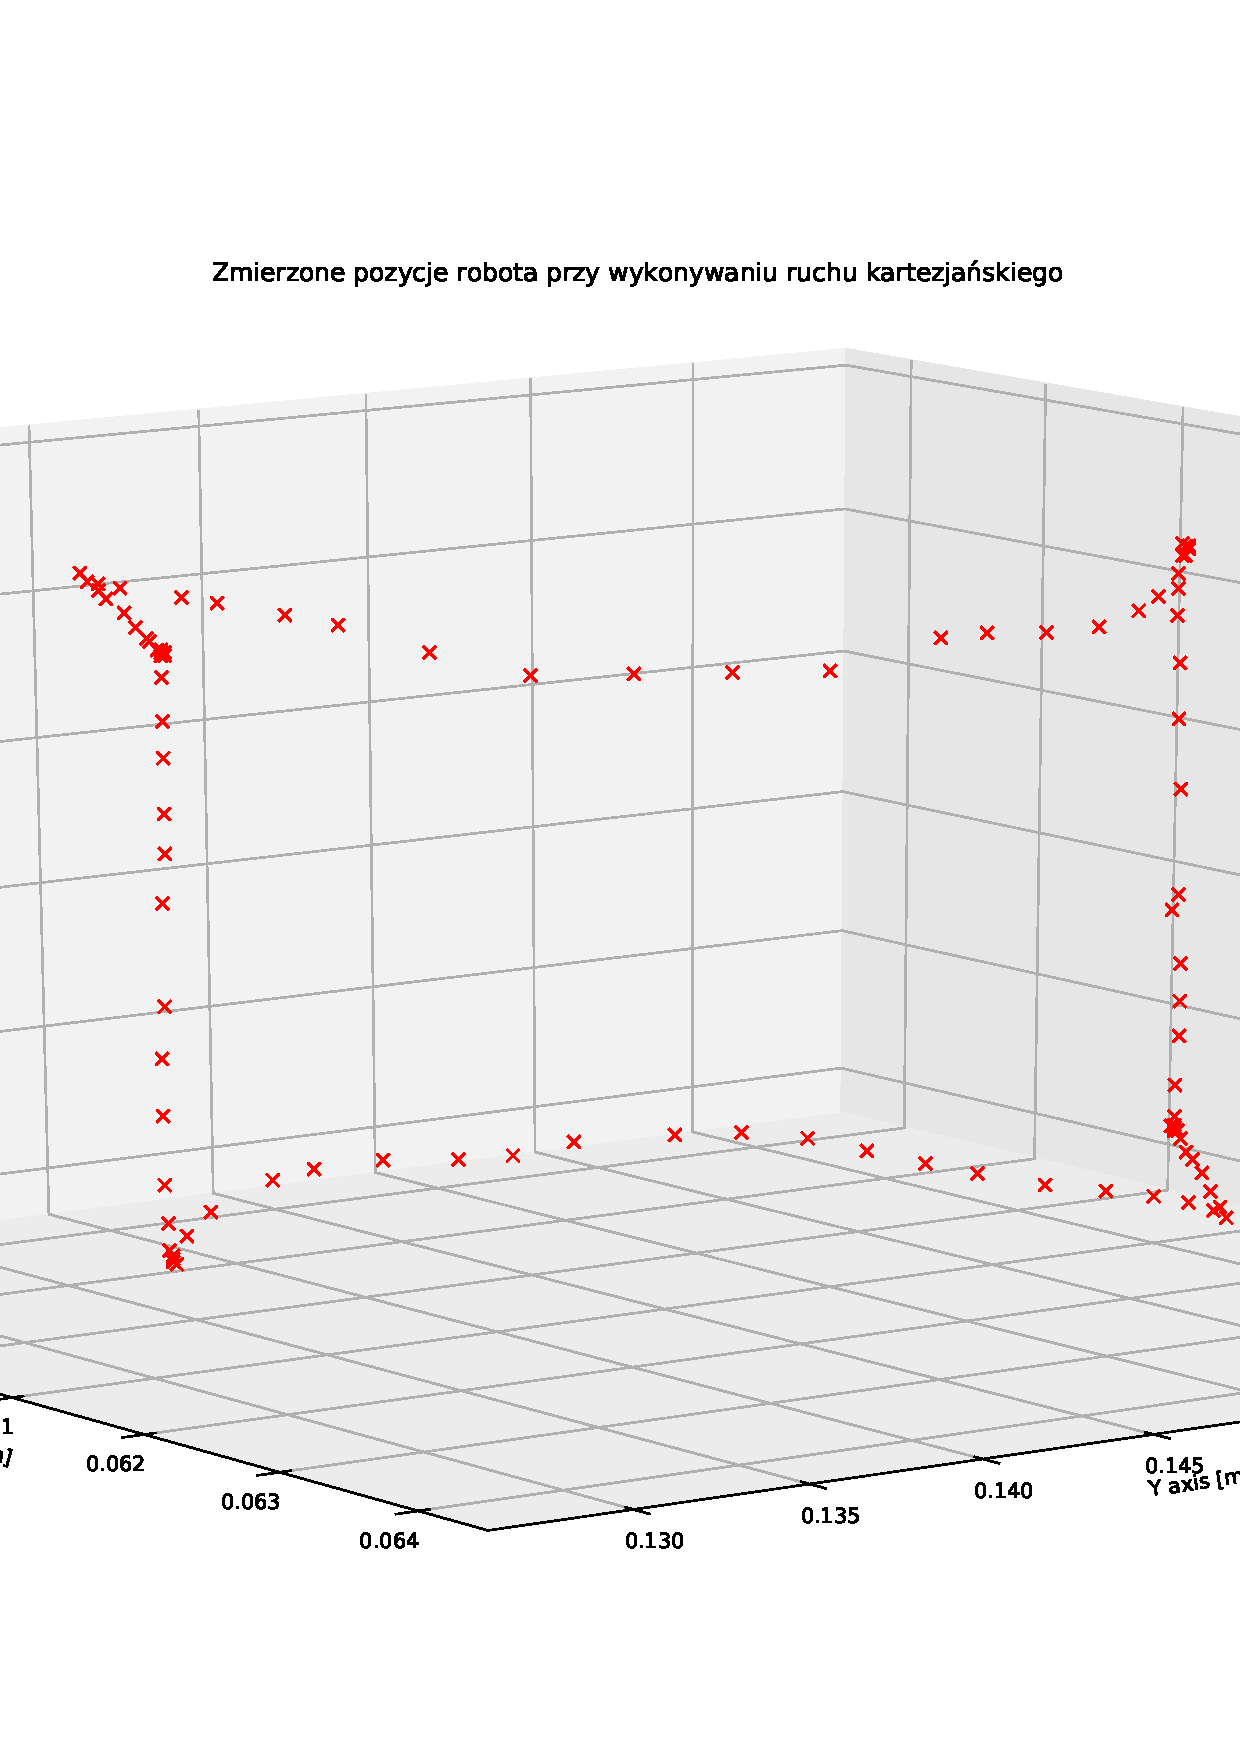
\includegraphics[width=1\linewidth]{{img/Figure_square.png}}
	\caption{Zaplanowana trajektoria przez planner dla realizacji przemieszczenia w układzie kartezjańskim. \cite{own}}
	\label{fig:37}
\end{figure}

Zaplanowano, iż ramię robota zakreśli czworokąt w płaszczyźnie pionowej. Napisano zatem węzeł - posłużywszy się językiem Python. Skrypt ten ładuje model robota z pliku URDF, następnie pobiera aktualny stan manipulatora, po czym nadsyła plannerowi kolejne punkty, które przyjęto na sztywno (wymiary czworokąta). \cite{Cart_file} 

Podobnie jak to miało miejsce wcześniej - tak i tym razem eksperymenty przeprowadzono zarówno dla symulacji w Gazebo jak i fizycznego robota. Powyżej zaprezentowano zaplanowaną przez planner trajektorię - rysunek \ref{fig:37}. Rysunek ten obrazuje również ideę przemieszczenia w układzie kartezjańskim. Jak widać pozycja złącza piątego (obrót chwytaka) zmienia się w taki sposób, iż stale utrzymywana jest konkretna płaszczyzna ruchu. Każdy punkt zaplanowany przez planner zaznaczono również niewielkim modelem układu współrzędnych, obrazującym orientację końcówki robota w przestrzeni. Można zauważyć iż jest ona stała. Takie zachowanie może być bardzo pożądane w niektórych zastosowaniach, takich jak wiercenie otworów, nakładanie warstwy kleju na szybę samochodu itp.  

Niemniej zaplanowana trasa jest trajektorią teoretyczną. Z tego też powodu rzeczywisty przebieg trajektorii robota zależy od jakości i precyzji jego wykonania. Dlatego poniżej zestawiono przestrzennie punkty pobrane w czasie symulowania ruchu manipulatora w programie Gazebo oraz z rzeczywistego urządzenia - \ref{fig:12}.  


\begin{figure}[H]
	\centering
	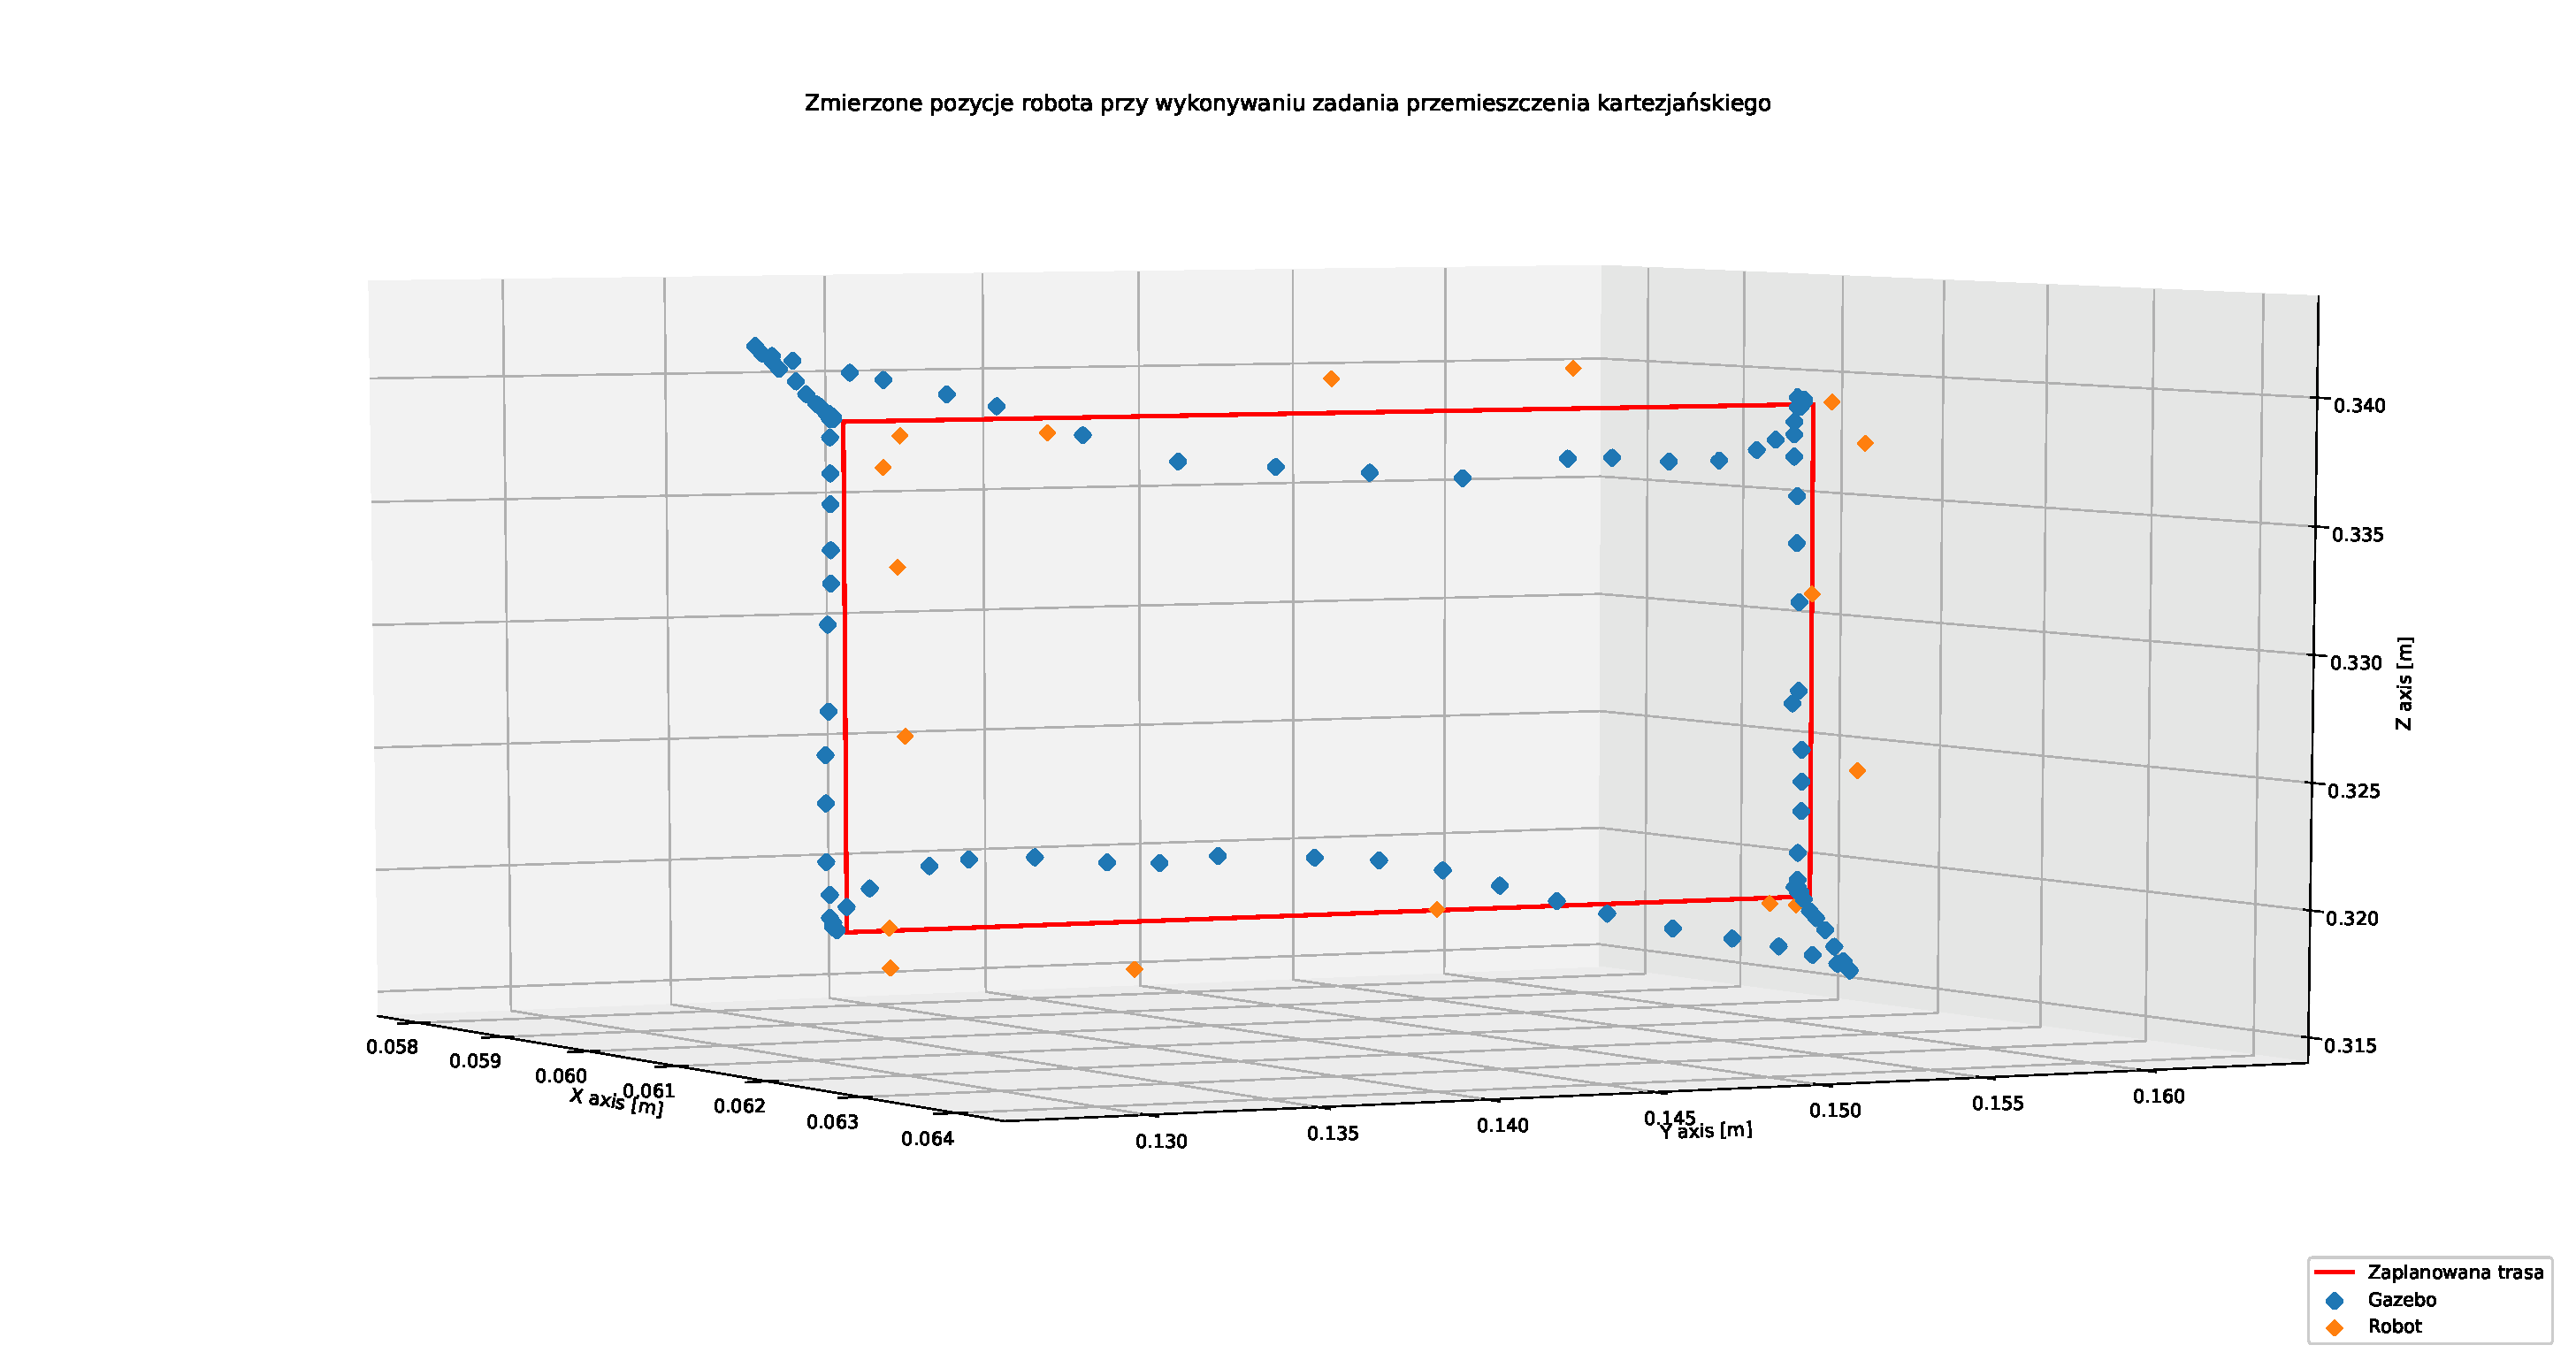
\includegraphics[width=1\linewidth]{{img/Figure_cartesian.eps}}
	\caption{Zmierzone pozycje robota przy wykonywaniu ruchu kartezjańskiego. \cite{own}}
	\label{fig:12}
\end{figure}

Jak widać w obu przypadkach trasa nie była idealna. Powodem, dla którego przebieg Gazebo znacznie odbiegał od pożądanego, były nastawy regulatora PID. W tym miejscu należy nadmienić, iż nastawy te należy dobrać zgodnie z masą oraz inercją złącz uwzględnioną w pliku URDF. Wartości te czerpano z fizycznych parametrów robota, niemniej po złym dobraniu nastawa regulatora (zbyt dużych bądź zbyt małych) w stosunku do opisanej fizyki robota, skutkuje przeróżnymi 'artefaktami' po uruchomieniu symulacji.

Jeżeli chodzi o wyniki rzeczywistego robota, to powody nieidealności jego przebiegu opisywano już wcześniej.

Dla końcowe podsumowania niniejszego eksperymentu, w poniższej tabeli zestawiono minimalne, maksymalne i średnie odchylenia od zaplanowanej trasy.


\begin{table}[H]
\centering
\caption{Porównanie odchyleń zmierzonych punktów robota w czasie wykonywania zadania przemieszczenia kartezjańskiego}
\label{tab:19}
\begin{tabular}{|c|c|c|c|c|}
\hline
\rowcolor[HTML]{C0C0C0} 
Lp & Model  & \begin{tabular}[c]{@{}c@{}}Min.\\ odchyłka\\ {[}m{]}\end{tabular} & \cellcolor[HTML]{C0C0C0}\begin{tabular}[c]{@{}c@{}}Max.\\ odchyłka\\ {[}m{]}\end{tabular} & \begin{tabular}[c]{@{}c@{}}Śr.\\ odchyłka\\ {[}m{]}\end{tabular} \\ \hline
\rowcolor[HTML]{FFCCC9} 
1. & Gazebo & 0.00051                                                           & 0.00866                                                                                   & 0.01181                                                          \\ \hline
\rowcolor[HTML]{9AFF99} 
2. & Robot  & 0.00054                                                           & 0.00139                                                                                   & 0.00210                                                          \\ \hline
\end{tabular}
\end{table}

W tym przypadku dokładniejszy okazał się fizyczny robot, niemniej jak wcześniej wspominano, jest to powiązane z nastawami regulatora.

Podsumowując przedstawione w niniejszym podrozdziale eksperymenty, można stwierdzić iż MoveIt nadaje się do generowania złożonych trajektorii i wykonywania przez manipulator konkretnych zadań. Wyznaczane trasy zależą jedynie od wyobraźni użytkownika oraz możliwości samego urządzenia. Jeżeli natomiast chodzi o otrzymane rezultaty związane z dokładnością odzwierciedlenia trasy, to nie były one idealne, jednak uwypukliły wrażliwe kwestie. Wiedza ta może zostać wykorzystana przy budowie kolejnych urządzeń bądź obsługi innych robotów.

\subsection{Sterowanie kartezjańskie i złączowe}

Zagadnieniem, które zdecydowano się również opisać jest różnica w ustalaniu nowej pozycji robota w programie Rviz, po modyfikacji parametru $position_only_ik$ pliku konfiguracyjnego $kinematics.yaml$. Parametr ten można ustawić na $True$ bądź $False$. Warunkuje on wyznaczanie nowych pozycji. W momencie gdy jest zanegowany wówczas użytkownik może modyfikować jedynie pozycje złącz. W momencie gdy został włączony wtedy wyznacza się pozycję robota w przestrzeni, do której ma zostać przesunięty, a nie samych osi. Wówczas też możliwe jest po prostu chwycenie myszką za interaktywny marker obecny na końcówce manipulatora i ustalenie nowej pozycji. W przypadku gdy włączone jest pozycjonowanie złącz opcja ta jest niemożliwa do wykonania. 



\begin{comment}


Jako że MoveIt wraz z ROSem udostępnia różne formy sterowania złączami w czasie realizacji trasy, toteż w tym podpunkcie postanowiono przetestować różnice w ich działaniu. \cite{Controllers}

Ze względu na uniwersalność oprogramowania ROS, pozwala on na sterowanie urządzeniami wykorzystującymi różne sposoby kontroli złącz. Oczywiście użytkownik może napisać swój dowolny sterownik, niemniej ROS domyślnie udostępnia trzy podstawowe.

Pierwszym z nich jest $Effort$ $Joint$ $Interface$ - dedykowany jest on robotom, których złącza sterowane są poprzez wartość siły, bądź momentu obrotowego.

Drugi - $Velocity$ $Joint$ $Interface$ - jak nazwa wskazuje jest przeznaczony do osi kontrolowanych przez określanie posiomu ich prędkości.

Ostatnim typem jest $Position$ $Joint$ $Interface$. W tym przypadku mowa o robotach, w których istotna jest jedynie pozycja danego członu.

Zatem postanowiono sprawdzić, jak różnią się sterowania oraz wiadomości wysyłane przez kontroler.


 \begin{figure}[H]
	\centering
	\includegraphics[width=0.9\linewidth]{{img/Figure_trajector.png}}
	\caption{Trajektoria poruszania się końcówki robota w czasie ruchu (DO WYMIANY, TYLKO TYP WYKRESU TEN SAM)}
	\label{fig:10}
\end{figure}


\subsection{Porównanie pluginów}

W czasie konfigurowania modelu robota w Setup Asisstant możliwy jest wybór pluginu, który będzie wykorzystywany na etapie rozwiązywania zadania kinematyki odwrotnej. Pierwszy z pluginów - $KDL Kinematics Plugin$ jest domyślny. Drugi - $LMA Kinematics Plugin$. Obie wtyczki posiadają podobne właściwości, gdyż w obu przypadkach opakowują one (ang. $wraps$) solvery kinematyki odwrotnej dostarczane przez paczkę $Orocos$ $KDL$. Oba pluginy zwracają uwagę na ograniczenia nałożone na poszczególne złącza, określone w plikach URDF. 

Postanowiono w związku z tym czy istnieje różnica w sposobie realizacji ruchu bądź planowania samej trasy między tymi dwoma pluginami. 

\cite{Plan_KDL_LMA}




\subsection{Ustawienia dodatkowe MoveIt}

Jako iż w programie Rviz, wtyczka MoveIt pozwala na określenie pewnych dodatkowych ustawień związanych z planowaniem oraz realizacją trasy, toteż postaniowo przetestować w jakim stopniu wpływają ustawienia te na proces wyznaczania trajektorii oraz jej bezpośrednią realizację.
Zatem użytkownik do dyspozycji posiada następujące ustawienia:
- $Use$ $Cartesian$ $Path$ - opcji tej należy użyć do wygenerowania liniwej trasy w przestrzeni kartezjańskiej. Opcja ta uniemożliwia planowania wokół przeszkód. Po jej zaznaczeniu uzyskano następujące rezultaty.


- $Colision$ $Avare$ $IK$ - 

- $Approx$ $IKSolutions$ - opcja ta dopuszcza przybliżone rozwiązania kinematyki odwrotnej, co jest przydatne w przypadku gdy punkt docelowy jest nieosiągalny. Po włączeniu tej opcji uzyskano:

- $External$ $ comm.$ - opcja ta udostępnia możliwość ustawiania punktów początkowych oraz końcowych jak również planowanie i wykonywanie trasy z poziomu zewnętrznych modułów. W tym celu konieczne jest po prostu wykorzystanie tematu /rviz/moveit.

Dwie kolejne opcje należą do grupy eksperymentalnych.
- $Replaning$ - opcja ta mogła zadziałać jedynie w przypadku uruchomienia komendy $Plan&Execute$, tj. gdy po planowaniu natychmiast następuje wykonanie trasy. W momencie gdy w czasie trwania ruchu zostanie wykryta kolizja, wtedy też trasa jest przeliczana na nowo.

- $Sensor$ $Positioning$ - była to ostatnia z opcji możliwa do użycia. Pozwala ona robotowi na zmianę pozycji swoich czujników, tak by możliwe było uniknięcie kolizji. (chyba to wywalę)


\subsection{Sposób ruchu złącz}

Głównym założeniem przyświecającym realizacji niniejszych eksperymentów było sprawdzenie, jak w czasie zmieniają się prędkości złącz przy realizacji ruchu. 
W tym celu zapisano ciągi sterowań wysyłane przez kontroler po czym najciekawsze przebiegi zestawiono zamieszczonych na wykresach. 



 \begin{figure}[H]
	\centering
	\includegraphics[width=0.8\linewidth]{{img/Figure_cartesian_2.png}}
	\caption{Zmierzone pozycje robota przy wykonywaniu ruchu kartezjańskiego (MOŻE DO WYMIANY)}
	\label{fig:13}
\end{figure}

 \begin{figure}[H]
	\centering
	\includegraphics[width=0.8\linewidth]{{img/Figure_PaP.eps}}
	\caption{Zmierzone pozycje robota przy wykonywaniu ruchu kartezjańskiego (MOŻE DO WYMIANY)}
	\label{fig:14}
\end{figure}

\clearpage

\section{Testy dokładności (accuracy)}



\section{Testy powtarzalności (repeability)}

\section{Omijanie przeszkód}

Kolejnym z zaproponowanych testów było sprawdzenie czy dany planner jest w stanie omijać przeszkody a także w jaki sposób to czyni. W czasie różnych eksperymentów dało się zauważyć, że niektóre 
 z zaplanowanych tras są w znacznym stopniu nieoptymalne. Toteż postanowiono się przyjrzeń również tym aspektom. 

 W tym celu postanowiono napisać dodatkowy skrypt w języku python, którego glównym zadaniem było liczenie długości drogi kątowej jaką musiało pokonać poszczególne złącze, a także jak to się prezentowało sumarycznie. 


 % Please add the following required packages to your document preamble:
% \usepackage{multirow}
% \usepackage[table,xcdraw]{xcolor}
% If you use beamer only pass "xcolor=table" option, i.e. \documentclass[xcolor=table]{beamer}
\begin{table}[H]
\caption{Porównanie czasów planowania poszczególnych algorytmów}
\label{tab:4}
\begin{tabular}{|c|c|c|c|c|c|c|ll}
\cline{1-7}
\cellcolor[HTML]{C0C0C0}L.p. & \cellcolor[HTML]{C0C0C0}{\color[HTML]{000000} \begin{tabular}[c]{@{}c@{}}Grupa \\ plannerów\end{tabular}} & \cellcolor[HTML]{C0C0C0}Planner     & \cellcolor[HTML]{C0C0C0}\begin{tabular}[c]{@{}c@{}}Min. zapla. \\ trasa {[}rad{]}\end{tabular} & \cellcolor[HTML]{C0C0C0}\begin{tabular}[c]{@{}c@{}}Max. zapla.\\  trasa {[}rad{]}\end{tabular} & \cellcolor[HTML]{C0C0C0}\begin{tabular}[c]{@{}c@{}}Średnia\\  trasy {[}rad{]}\end{tabular} & \cellcolor[HTML]{C0C0C0}Uwagi &  &  \\ \cline{1-7}
\cellcolor[HTML]{EFEFEF}1.   & CHOMP                                                                                                     & \cellcolor[HTML]{EFEFEF}CHOMP       & \cellcolor[HTML]{EFEFEF}                                                                       & \cellcolor[HTML]{EFEFEF}                                                                       & \cellcolor[HTML]{EFEFEF}                                                                   & \cellcolor[HTML]{EFEFEF}      &  &  \\ \cline{1-7}
\cellcolor[HTML]{C0C0C0}2.   &                                                                                                           & \cellcolor[HTML]{C0C0C0}BFMT        & \cellcolor[HTML]{C0C0C0}                                                                       & \cellcolor[HTML]{C0C0C0}                                                                       & \cellcolor[HTML]{C0C0C0}                                                                   & \cellcolor[HTML]{C0C0C0}      &  &  \\ \cline{1-1} \cline{3-7}
\cellcolor[HTML]{EFEFEF}3.   &                                                                                                           & \cellcolor[HTML]{EFEFEF}BKPIECE     & \cellcolor[HTML]{EFEFEF}                                                                       & \cellcolor[HTML]{EFEFEF}                                                                       & \cellcolor[HTML]{EFEFEF}                                                                   & \cellcolor[HTML]{EFEFEF}      &  &  \\ \cline{1-1} \cline{3-7}
\cellcolor[HTML]{C0C0C0}4.   &                                                                                                           & \cellcolor[HTML]{C0C0C0}BiEST       & \cellcolor[HTML]{C0C0C0}                                                                       & \cellcolor[HTML]{C0C0C0}                                                                       & \cellcolor[HTML]{C0C0C0}                                                                   & \cellcolor[HTML]{C0C0C0}      &  &  \\ \cline{1-1} \cline{3-7}
\cellcolor[HTML]{EFEFEF}5.   &                                                                                                           & \cellcolor[HTML]{EFEFEF}BiTRRT      & \cellcolor[HTML]{EFEFEF}                                                                       & \cellcolor[HTML]{EFEFEF}                                                                       & \cellcolor[HTML]{EFEFEF}                                                                   & \cellcolor[HTML]{EFEFEF}      &  &  \\ \cline{1-1} \cline{3-7}
\cellcolor[HTML]{C0C0C0}6.   &                                                                                                           & \cellcolor[HTML]{C0C0C0}EST         & \cellcolor[HTML]{C0C0C0}                                                                       & \cellcolor[HTML]{C0C0C0}                                                                       & \cellcolor[HTML]{C0C0C0}                                                                   & \cellcolor[HTML]{C0C0C0}      &  &  \\ \cline{1-1} \cline{3-7}
\cellcolor[HTML]{EFEFEF}7.   &                                                                                                           & \cellcolor[HTML]{EFEFEF}FMT         & \cellcolor[HTML]{EFEFEF}                                                                       & \cellcolor[HTML]{EFEFEF}                                                                       & \cellcolor[HTML]{EFEFEF}                                                                   & \cellcolor[HTML]{EFEFEF}      &  &  \\ \cline{1-1} \cline{3-7}
\cellcolor[HTML]{C0C0C0}8.   &                                                                                                           & \cellcolor[HTML]{C0C0C0}KPIECE      & \cellcolor[HTML]{C0C0C0}                                                                       & \cellcolor[HTML]{C0C0C0}                                                                       & \cellcolor[HTML]{C0C0C0}                                                                   & \cellcolor[HTML]{C0C0C0}      &  &  \\ \cline{1-1} \cline{3-7}
\cellcolor[HTML]{EFEFEF}9.   &                                                                                                           & \cellcolor[HTML]{EFEFEF}LBKPIECE    & \cellcolor[HTML]{EFEFEF}                                                                       & \cellcolor[HTML]{EFEFEF}                                                                       & \cellcolor[HTML]{EFEFEF}                                                                   & \cellcolor[HTML]{EFEFEF}      &  &  \\ \cline{1-1} \cline{3-7}
\cellcolor[HTML]{C0C0C0}10.  &                                                                                                           & \cellcolor[HTML]{C0C0C0}LBTRRT      & \cellcolor[HTML]{C0C0C0}                                                                       & \cellcolor[HTML]{C0C0C0}                                                                       & \cellcolor[HTML]{C0C0C0}                                                                   & \cellcolor[HTML]{C0C0C0}      &  &  \\ \cline{1-1} \cline{3-7}
\cellcolor[HTML]{EFEFEF}11.  &                                                                                                           & \cellcolor[HTML]{EFEFEF}LazyPRM     & \cellcolor[HTML]{EFEFEF}                                                                       & \cellcolor[HTML]{EFEFEF}                                                                       & \cellcolor[HTML]{EFEFEF}                                                                   & \cellcolor[HTML]{EFEFEF}      &  &  \\ \cline{1-1} \cline{3-7}
\cellcolor[HTML]{C0C0C0}12.  &                                                                                                           & \cellcolor[HTML]{C0C0C0}LazyPRMstar & \cellcolor[HTML]{C0C0C0}                                                                       & \cellcolor[HTML]{C0C0C0}                                                                       & \cellcolor[HTML]{C0C0C0}                                                                   & \cellcolor[HTML]{C0C0C0}      &  &  \\ \cline{1-1} \cline{3-7}
\cellcolor[HTML]{EFEFEF}13.  &                                                                                                           & \cellcolor[HTML]{EFEFEF}PDST        & \cellcolor[HTML]{EFEFEF}                                                                       & \cellcolor[HTML]{EFEFEF}                                                                       & \cellcolor[HTML]{EFEFEF}                                                                   & \cellcolor[HTML]{EFEFEF}      &  &  \\ \cline{1-1} \cline{3-7}
\cellcolor[HTML]{C0C0C0}14.  &                                                                                                           & \cellcolor[HTML]{C0C0C0}PRM         & \cellcolor[HTML]{C0C0C0}                                                                       & \cellcolor[HTML]{C0C0C0}                                                                       & \cellcolor[HTML]{C0C0C0}                                                                   & \cellcolor[HTML]{C0C0C0}      &  &  \\ \cline{1-1} \cline{3-7}
\cellcolor[HTML]{EFEFEF}15.  &                                                                                                           & \cellcolor[HTML]{EFEFEF}PRMstar     & \cellcolor[HTML]{EFEFEF}                                                                       & \cellcolor[HTML]{EFEFEF}                                                                       & \cellcolor[HTML]{EFEFEF}                                                                   & \cellcolor[HTML]{EFEFEF}      &  &  \\ \cline{1-1} \cline{3-7}
\cellcolor[HTML]{C0C0C0}16.  &                                                                                                           & \cellcolor[HTML]{C0C0C0}ProjEST     & \cellcolor[HTML]{C0C0C0}                                                                       & \cellcolor[HTML]{C0C0C0}                                                                       & \cellcolor[HTML]{C0C0C0}                                                                   & \cellcolor[HTML]{C0C0C0}      &  &  \\ \cline{1-1} \cline{3-7}
\cellcolor[HTML]{EFEFEF}11.  &                                                                                                           & \cellcolor[HTML]{EFEFEF}RRTConnect  & \cellcolor[HTML]{EFEFEF}                                                                       & \cellcolor[HTML]{EFEFEF}                                                                       & \cellcolor[HTML]{EFEFEF}                                                                   & \cellcolor[HTML]{EFEFEF}      &  &  \\ \cline{1-1} \cline{3-7}
\cellcolor[HTML]{C0C0C0}12.  &                                                                                                           & \cellcolor[HTML]{C0C0C0}RRT         & \cellcolor[HTML]{C0C0C0}                                                                       & \cellcolor[HTML]{C0C0C0}                                                                       & \cellcolor[HTML]{C0C0C0}                                                                   & \cellcolor[HTML]{C0C0C0}      &  &  \\ \cline{1-1} \cline{3-7}
\cellcolor[HTML]{EFEFEF}13.  &                                                                                                           & \cellcolor[HTML]{EFEFEF}RRTstar     & \cellcolor[HTML]{EFEFEF}                                                                       & \cellcolor[HTML]{EFEFEF}                                                                       & \cellcolor[HTML]{EFEFEF}                                                                   & \cellcolor[HTML]{EFEFEF}      &  &  \\ \cline{1-1} \cline{3-7}
\cellcolor[HTML]{C0C0C0}14.  &                                                                                                           & \cellcolor[HTML]{C0C0C0}SBL         & \cellcolor[HTML]{C0C0C0}                                                                       & \cellcolor[HTML]{C0C0C0}                                                                       & \cellcolor[HTML]{C0C0C0}                                                                   & \cellcolor[HTML]{C0C0C0}      &  &  \\ \cline{1-1} \cline{3-7}
\cellcolor[HTML]{EFEFEF}15.  &                                                                                                           & \cellcolor[HTML]{EFEFEF}SPARS       & \cellcolor[HTML]{EFEFEF}                                                                       & \cellcolor[HTML]{EFEFEF}                                                                       & \cellcolor[HTML]{EFEFEF}                                                                   & \cellcolor[HTML]{EFEFEF}      &  &  \\ \cline{1-1} \cline{3-7}
\cellcolor[HTML]{C0C0C0}16.  &                                                                                                           & \cellcolor[HTML]{C0C0C0}SPARStwo    & \cellcolor[HTML]{C0C0C0}                                                                       & \cellcolor[HTML]{C0C0C0}                                                                       & \cellcolor[HTML]{C0C0C0}                                                                   & \cellcolor[HTML]{C0C0C0}      &  &  \\ \cline{1-1} \cline{3-7}
\cellcolor[HTML]{EFEFEF}17.  &                                                                                                           & \cellcolor[HTML]{EFEFEF}STRIDE      & \cellcolor[HTML]{EFEFEF}                                                                       & \cellcolor[HTML]{EFEFEF}                                                                       & \cellcolor[HTML]{EFEFEF}                                                                   & \cellcolor[HTML]{EFEFEF}      &  &  \\ \cline{1-1} \cline{3-7}
\cellcolor[HTML]{C0C0C0}18.  & \multirow{-23}{*}{OMPL}                                                                                   & \cellcolor[HTML]{C0C0C0}TRRT        & \cellcolor[HTML]{C0C0C0}                                                                       & \cellcolor[HTML]{C0C0C0}                                                                       & \cellcolor[HTML]{C0C0C0}                                                                   & \cellcolor[HTML]{C0C0C0}      &  &  \\ \cline{1-7}
\cellcolor[HTML]{EFEFEF}19.  &                                                                                                           & \cellcolor[HTML]{EFEFEF}PTP         & \cellcolor[HTML]{EFEFEF}                                                                       & \cellcolor[HTML]{EFEFEF}                                                                       & \cellcolor[HTML]{EFEFEF}                                                                   & \cellcolor[HTML]{EFEFEF}      &  &  \\ \cline{1-1} \cline{3-7}
\cellcolor[HTML]{C0C0C0}20.  & \multirow{-2}{*}{\begin{tabular}[c]{@{}c@{}}Pilz Industrial \\ \\ Motion Planner\end{tabular}}            & \cellcolor[HTML]{C0C0C0}LIN         & \cellcolor[HTML]{C0C0C0}                                                                       & \cellcolor[HTML]{C0C0C0}                                                                       & \cellcolor[HTML]{C0C0C0}                                                                   & \cellcolor[HTML]{C0C0C0}      &  &  \\ \cline{1-7}
\end{tabular}
\end{table}

\end{comment}

\section{Podsumowanie rozdziału}

Podsumowując przeprowadzone w niniejszym rozdziale liczne testy, można stwierdzić iż MoveIt udostępnia użytkownikom spory zakres funkcjonalności. Liczba możliwych do użycia plannerów, opcji, sposobów poruszania, jest znaczna. Rozwiązanie problemu kinematyki odwrotnej nie jest zadaniem prostym, jednak MoveIt posiada solvery takie wbudowane w siebie. Pozwala to na znaczące skrócenie czasu rozwoju projektu nowego robota. Musząc samemu stworzyć planner trajektorii, prawdopodobnie zrealizowano by to mało optymalnie. MoveIt nie tylko udostępnia takie rozwiązania gotowe, co również pozwala na wybieranie między nimi. W ten sposób można skupić się jedynie na kwestii obierania sygnałów sterujących od MoveIta i ich odpowiednie przetwarzanie bezpośrednio na wymagane ruchy silników.

Na pewno korzystanie z ROSa wprowadza pewne ograniczenia, narzuca pewne standardy, niemniej możliwości konfiguracyjne oraz edytorskie są na tyle duże, iż praktycznie każdą funkcjonalność, która w pewnym stopniu użytkownikowi nie odpowiada można zmodfikować badź po prostu napisać własną.

